% !TEX program = xelatex
% !TEX root = main.tex


\documentclass[12pt]{article}

% --- Hyperlinks ---
\usepackage{hyperref}
\hypersetup{
	breaklinks=true
}

% --- Layout & Formatting ---
\usepackage{ragged2e}
\usepackage{graphicx}
\graphicspath{{figures/}}
\usepackage{float}
\usepackage{lipsum}  % For dummy text
\newcommand{\ignore}[1]{}

% --- Math & Symbols ---
\usepackage{amsmath}
\usepackage{amssymb}
\usepackage{eurosym}

% --- Fonts & Language (XeLaTeX / LuaLaTeX) ---
\usepackage{fontspec}
\usepackage{polyglossia}

% Set languages
\setmainlanguage{greek}
\setotherlanguage{english}

% Explicitly set font families that support the Greek script
% You can use system fonts like "Times New Roman" / "Arial", 
% or free TeX fonts like Noto / FreeSerif / Linux Libertine.
\setmainfont{Noto Serif}[Script=Greek]
\setsansfont{Noto Sans}[Script=Greek]
\setmonofont{Noto Sans Mono}[Script=Greek]

\usepackage{geometry}
\geometry{
  a4paper,
  left=20mm,
  top=20mm,
  right=20mm,
  bottom=20mm
}

\usepackage{fancyhdr}

\fancypagestyle{plain}{
    \fancyhf{}
    \rfoot{\thepage}
}

\fancyhf{}
\renewcommand{\headrulewidth}{0pt}
\fancyfoot[R]{\thepage}

\pagestyle{fancy}

% Paragraph spacing
\setlength{\parindent}{3em}
\setlength{\parskip}{.8em}
\renewcommand{\baselinestretch}{1.2}

\usepackage{titlesec}

\makeatletter
\@addtoreset{section}{part}
\makeatother
\titleformat{\part}[display]
{\normalfont\LARGE\bfseries\centering}{}{0pt}{}

\usepackage{setspace}
\setstretch{1.5}

\usepackage{graphicx}

\renewcommand{\refname}{Αναφορές}

\begin{document}

\thispagestyle{empty}
  \begin{center}
  \begin{tabular}{cc}
  
\includegraphics[scale=0.27]{hua.png} &
  \begin{minipage}{.7\linewidth}
    \vspace{-1.5cm}
        {\fontsize{24}{24} \textbf{ΧΑΡΟΚΟΠΕΙΟ ΠΑΝΕΠΙΣΤΗΜΙΟ}}
  \end{minipage}\\
  \end{tabular}

  {\vspace{0.5cm}\fontsize{16}{16}\selectfont ΣΧΟΛΗ ΨΗΦΙΑΚΗΣ ΤΕΧΝΟΛΟΓΙΑΣ}\\
    \vspace{0.15cm}
  {\fontsize{16}{16}\selectfont ΤΜΗΜΑ ΠΛΗΡΟΦΟΡΙΚΗΣ ΚΑΙ ΤΗΛΕΜΑΤΙΚΗΣ}\\
    \vspace{5cm}
  {\fontsize{14}{14}\selectfont \textbf{ΤΙΤΛΟΣ ΕΡΓΑΣΙΑΣ}}\\
  {\fontsize{14}{14}\selectfont Μελέτη και αξιολόγηση σύγχρονων μεθόδων τεχνητής νοημοσύνης για πράκτορες παιχνιδιών
  }\\
    \vspace{0.43cm}
  {\fontsize{14}{14}\selectfont \textbf{ΟΝΟΜΑ ΕΠΩΝΥΜΟ}}\\
  {\fontsize{14}{14}\selectfont Ορέστης Αποστόλου
  }\\
  \vspace*{\fill}
  {\fontsize{14}{14}\selectfont Αθήνα, 2026}\\

  \end{center}
\pagebreak

\thispagestyle{plain}
  \begin{center}
  \begin{tabular}{cc}
  
\includegraphics[scale=0.27]{hua.png} &
  \begin{minipage}{.7\linewidth}
    \vspace{-1.5cm}
        {\fontsize{24}{24} \textbf{HAROKOPIO UNIVERSITY}}
  \end{minipage}\\
  \end{tabular}

  {\vspace{0.5cm}\fontsize{16}{16}\selectfont SCHOOL OF DIGITAL TECHNOLOGY}\\
    \vspace{0.15cm}
  {\fontsize{16}{16}\selectfont DEPARTMENT OF INFORMATICS AND TELEMATICS}\\
    \vspace{5cm}
  {\fontsize{14}{14}\selectfont \textbf{TITLE}}\\
  {\fontsize{14}{14}\selectfont Bachelor Thesis}\\
    \vspace{0.43cm}
  {\fontsize{14}{14}\selectfont \textbf{NAME SURNAME}}\\
  {\fontsize{14}{14}\selectfont Orestis Apostolou
  }\\
  \vspace*{\fill}
  {\fontsize{14}{14}\selectfont Athens, 2026}\\

  \end{center}

\pagebreak
\thispagestyle{plain} 
  \begin{center}
  \begin{tabular}{cc}
  
\includegraphics[scale=0.27]{hua.png}
  &
  \begin{minipage}{.7\linewidth}
    \vspace{-1.5cm}
        {\fontsize{24}{24} \textbf{ΧΑΡΟΚΟΠΕΙΟ ΠΑΝΕΠΙΣΤΗΜΙΟ}}
  \end{minipage}
  \end{tabular}
  \\
  {\vspace{0.5cm} \fontsize{16}{16}\selectfont ΣΧΟΛΗ ΨΗΦΙΑΚΗΣ ΤΕΧΝΟΛΟΓΙΑΣ}
    \vspace{0.15cm}
    \\
  {\fontsize{16}{16}\selectfont ΤΜΗΜΑ ΠΛΗΡΟΦΟΡΙΚΗΣ ΚΑΙ ΤΗΛΕΜΑΤΙΚΗΣ}\\
        \vspace{3cm}
    {\fontsize{16}{16}\selectfont \textbf{Τριμελής Εξεταστική Επιτροπή}}\\[1\baselineskip]
    {\fontsize{14}{14}\selectfont \textbf{Χρήστος Δίου (Επιβλέπων)\\
    Αναπληρωτής Καθηγητής, Πληροφορικής και Τηλεματικής, \\Χαροκόπειο Πανεπιστήμιο}}\\[1\baselineskip]

    {\fontsize{14}{14}\selectfont \textbf{Άγγελος Χαραλαμπίδης\\
    Επίκουρος Καθηγητής, Πληροφορικής και Τηλεματικής, \\Χαροκόπειο Πανεπιστήμιο}}\\[1\baselineskip]

    {\fontsize{14}{14}\selectfont \textbf{Βασίλης Ευθυμίου\\
    Επίκουρος Καθηγητής, Πληροφορικής και Τηλεματικής, \\Χαροκόπειο Πανεπιστήμιο}}\\
   
  \end{center}

\pagebreak
\thispagestyle{plain}

{\fontsize{14}{14}\selectfont
Ο ....... , δηλώνω υπεύθυνα ότι:

\begin{enumerate}
\item Είμαι ο κάτοχος των πνευματικών δικαιωμάτων της πρωτότυπης αυτής εργασίας και από όσο γνωρίζω η εργασία μου δε συκοφαντεί πρόσωπα, ούτε προσβάλει τα πνευματικά δικαιώματα τρίτων.
\item Αποδέχομαι ότι η ΒΚΠ μπορεί, χωρίς να αλλάξει το περιεχόμενο της εργασίας μου, να τη διαθέσει σε ηλεκτρονική μορφή μέσα από τη ψηφιακή Βιβλιοθήκη της, να την αντιγράψει σε οποιοδήποτε μέσο ή/και σε οποιοδήποτε μορφότυπο καθώς και να κρατά περισσότερα από ένα αντίγραφα για λόγους συντήρησης και ασφάλειας.
\item Όπου υφίστανται δικαιώματα άλλων δημιουργών έχουν διασφαλιστεί όλες οι αναγκαίες άδειες χρήσης ενώ το αντίστοιχο υλικό είναι ευδιάκριτο στην υποβληθείσα εργασία.
\end{enumerate}
}

\pagebreak
\thispagestyle{plain}
\vspace*{\fill}
\begin{flushright}
{\fontsize{14}{14}\selectfont
\textit{Αφιερωμένο ....}
}
\end{flushright}
\vspace*{\fill}

\pagebreak
\thispagestyle{plain}
\begin{center}
{\fontsize{16}{16}\selectfont \underline{\textbf{ΕΥΧΑΡΙΣΤΙΕΣ}}}
\end{center}
\vspace{1cm}

Με βαθιά ευγνωμοσύνη, θα ήθελα να ευχαριστήσω τον επιβλέποντα καθηγητή μου, κ. Χρήστο Δίου για την ουσιαστική καθοδήγηση και την υποστήριξη που μου παρείχε καθ' όλη τη διάρκεια της εκπόνησης της παρούσας εργασίας. 

Επίσης θα ήθελα να ευχαριστήσω τον αδερφό μου, που με εισήγαγε στον κόσμο των παιχνιδιών και, με το μεταδοτικό του ενδιαφέρον για τα Μαθηματικά και την Πληροφορική, με οδήγησε στην επιδίωξη πτυχίου στην Επιστήμη των Υπολογιστών.
\pagebreak


\renewcommand{\contentsname}{Πίνακας περιεχομένων}
\pagebreak
\begin{spacing}{1.3}
\tableofcontents
\end{spacing}

\pagebreak
\section*{Περίληψη στα Ελληνικά}
Η εργασία συγκρίνει παραδοσιακούς πράκτορες παιχνιδιών βασισμένους σε κανόνες
(Finite State Machine σε συνδυασμό με τον αλγόριθμο A*) με πράκτορες Ενισχυτικής
Μάθησης (Reinforcement Learning), εκπαιδευμένους με τον αλγόριθμο PPO, σε ένα
συμμετρικό, ανταγωνιστικό 2D περιβάλλον που αναπτύχθηκε στο Unity/ML-Agents.
Στο περιβάλλον αυτό, δύο πράκτορες μονομαχούν σε μια αρένα με δυναμικά,
τυχαία παραγόμενα εμπόδια (procedural generation), υπό ένα σύστημα πόντων ζωής,
βλημάτων και ελέγχου θερμοκρασίας πυρός.

Εξετάστηκαν πέντε πειραματικά σενάρια Ενισχυτικής Μάθησης με διάφορες μετρικές:
\begin{itemize}
	\item PPO εναντίον της απλής (baseline) εκδοχής του rule-based πράκτορα, σε 5 και 10 εκατομμύρια βήματα,
	\item PPO εναντίον της σύνθετης (advanced) εκδοχής του rule-based πράκτορα,
	\item PPO με εκπαίδευση self-play,
	\item PPO με fine-tuning του self-play πράκτορα εναντίον της απλής εκδοχής του rule-based πράκτορα.
\end{itemize}

Τα αποτελέσματα υποδεικνύουν ότι η Ενισχυτική Μάθηση αποτελεί μία πρακτική και ανταγωνιστική λύση για την ανάπτυξη πρακτόρων σε περιβάλλοντα παιχνιδιών με ελάχιστη ανθρώπινη προσπάθεια.

\vspace{5cm}
\noindent {\fontsize{14}{14}\selectfont \textbf{Λέξεις κλειδιά:}} ενισχυτική μάθηση, πράκτορες παιχνιδιών, αυτό-εκπαίδευση, πράκτορες βασισμένοι σε κανόνες

\pagebreak
\section*{Abstract ή Περίληψη στα Αγγλικά}

This thesis compares traditional rule-based game agents, built on a Finite
State Machine combined with the A* pathfinding algorithm, against
Reinforcement Learning agents trained with the Proximal Policy Optimization
(PPO) algorithm, within a symmetric, adversarial 2D combat environment
developed in Unity using ML-Agents. The environment features procedurally
generated, destructible obstacles, a health and resource-based shooting system,
and two agents competing under identical rules.

Several training approaches were evaluated, including PPO trained against
static rule-based opponents of varying difficulty, PPO trained through
self-play, and a subsequent fine-tuning phase applied to the self-play agent.
The results show that RL agents are capable of consistently outperforming
rule-based opponents while spontaneously developing behaviors typically
associated with hand-crafted agents, such as positioning, cover usage, and
projectile avoidance, without any explicit behavioral scripting and without
resorting to a time-consuming reward shaping process. Self-play training
further encouraged the emergence of active, generalizable targeting skills,
while a short fine-tuning phase against a static opponent substantially
improved both performance and generalization at minimal additional
computational cost.

Overall, the findings suggest that Reinforcement Learning constitutes a
practical and viable alternative to conventional rule-based approaches for
game agent development, capable of producing competent, adaptable agents
with comparatively little manual effort.

\vspace{8cm}
\noindent {\fontsize{14}{14}\selectfont \textbf{Keywords:}} reinforcement learning, PPO, game agents, self-play, rule-based agents, unity

\renewcommand{\listfigurename}{Κατάλογος εικόνων}
\pagebreak
\listoffigures

\pagebreak
\listoftables 

\pagebreak
\section*{Συντομογραφίες}
\begin{table}[ht]
\centering
\begin{tabular}{| c | c |}
\hline
REST    & Representational State Transfer \\
\hline
API     & Application Programming Interface \\
\hline
\end{tabular}
\end{table}

\pagebreak
\section{Εισαγωγή}
Η Τεχνητή Νοημοσύνη αποτελεί έναν από τους πιο δυναμικούς τομείς της Επιστήμης Υπολογιστών, με τον κλάδο της ενισχυτικής μάθησης (Reinforcement Learning - RL) να προσελκύει ιδιαίτερο ενδιαφέρον χάρη στις ραγδαίες αλγοριθμικές εξελίξεις του πεδίου. 

Οι εξελίξεις αυτές προσφέρουν νέες δυνατότητες για την αυτόνομη λήψη αποφάσεων και την προσαρμογή πρακτόρων (\foreignlanguage{english}{agents}) σε δυναμικά περιβάλλοντα. Διαχρονικό πεδίο δοκιμής και αξιολόγησης σχετικών αλγορίθμων αποτελούν τα περιβάλλοντα βιντεοπαιχνιδιών, στα οποία όμως στην πράξη, συνεχίζουν να επικρατούν κλασικοί πράκτορες βασισμένοι σε κανόνες (rule-based agents). Βασικοί λόγοι πίσω από αυτήν την επικράτηση είναι η σταθερότητα και η προβλεψιμότητα που προσφέρουν, παρά το γεγονός ότι απαιτούν χειρωνακτικό σχεδιασμό από τους προγραμματιστές και εμφανίζουν περιορισμένη προσαρμοστικότητα.

Στο πλαίσιο αυτό, τα συμμετρικά ανταγωνιστικά παιχνίδια \foreignlanguage{english}{(symmetric adversarial games)} προσφέρουν ένα δίκαιο και απαιτητικό πεδίο αξιολόγησης, όπου οι ενέργειες κάθε πράκτορα επιβάλλουν την άμεση προσαρμογή του αντιπάλου. Παράλληλα, η εισαγωγή ενός δυναμικού περιβάλλοντος ενισχύει το βάθος των αναπτυσσόμενων συμπεριφορών και τη γενικευσιμότητα των ικανοτήτων του αυτόνομου πράκτορα.

Αξιοποιώντας το παραπάνω περιβάλλον, η παρούσα εργασία θέτει ως στόχο τη σύγκριση παραδοσιακών τεχνικών Τεχνητής Νοημοσύνης παιχνιδιών με σύγχρονες μεθόδους Ενισχυτικής Μάθησης, εξετάζοντας τη βιωσιμότητα των δεύτερων υπό συνθήκες ελαχιστοποιημένης ανθρώπινης παρέμβασης κατά την εκπαίδευση του πράκτορα.

\section{Μεθοδολογία}
\subsection{Θεωρητικό Υπόβαθρο}
Στις ενότητες που ακολουθούν περιγράφεται το θεωρητικό υπόβαθρο που κρίνεται απαραίτητο για την κατανόηση των πειραμάτων, σχεδιαστικών αποφάσεων του περιβάλλοντος αξιολόγησης και χρησιμοποιούμενων μεθόδων της μελέτης.

\subsubsection{Μηχανές Πεπερασμένων Καταστάσεων}
Μία μηχανή πεπερασμένων καταστάσεων (Finite State Machine, FSM) αποτελεί ένα υπολογιστικό μοντέλο ευρέως χρησιμοποιούμενο για τη μοντελοποίηση της συμπεριφοράς πρακτόρων σε παιχνίδια, λόγω της ευελιξίας και απλότητας του. Μία FSM αποτελείται από ένα πεπερασμένο σύνολο καταστάσεων (states), εκ των οποίων ο πράκτορας βρίσκεται πάντα σε ακριβώς μία, και ένα σύνολο μεταβάσεων (transitions) μεταξύ καταστάσεων, οι οποίες ενεργοποιούνται όταν ικανοποιούνται συγκεκριμένες, ρητά ορισμένες συνθήκες (π.χ. απόσταση από τον αντίπαλο, επίπεδο πόντων ζωής). Κάθε κατάσταση αντιστοιχεί σε ένα διακριτό, καλά ορισμένο πρότυπο συμπεριφοράς (π.χ. αναζήτηση αντιπάλου, επίθεση, υποχώρηση), και ο πράκτορας εκτελεί τη συμπεριφορά που αντιστοιχεί στην τρέχουσα κατάστασή του μέχρι να πληρωθεί κάποια συνθήκη μετάβασης προς άλλη κατάσταση.

\subsubsection{Ο Αλγόριθμος A*}
Ο A* (A-star) είναι ένας κλασικός αλγόριθμος αναζήτησης σε γραφήματα, ευρέως χρησιμοποιούμενος για την εύρεση του βέλτιστου (ελάχιστου κόστους) μονοπατιού μεταξύ μιας αρχικής και μιας τελικής κατάστασης. Αποτελεί επέκταση του αλγορίθμου Dijkstra, ενσωματώνοντας πρόσθετη πληροφορία μέσω μιας ευρετικής συνάρτησης (heuristic function) που καθοδηγεί την αναζήτηση προς την κατεύθυνση του στόχου, καθιστώντας τον σημαντικά πιο αποδοτικό σε πρακτικές εφαρμογές.

Ο A* διατηρεί μια συνάρτηση αξιολόγησης $f(n)$ για κάθε κόμβο $n$ του χώρου αναζήτησης, η οποία ορίζεται ως $f(n) = g(n) + h(n)$, όπου:

\begin{itemize}
    \item $g(n)$ είναι το πραγματικό κόστος της διαδρομής από τον αρχικό κόμβο μέχρι τον κόμβο $n$,
    \item $h(n)$ είναι η ευρετική εκτίμηση του κόστους από τον κόμβο $n$ μέχρι τον τελικό κόμβο (στόχο),
    \item $f(n)$ είναι η συνολική εκτιμώμενη τιμή του κόμβου $n$, δηλαδή το εκτιμώμενο συνολικό κόστος μιας διαδρομής που περνάει από τον κόμβο $n$.
\end{itemize}

Σε κάθε βήμα, ο αλγόριθμος επιλέγει προς επέκταση τον κόμβο με τη μικρότερη τιμή $f(n)$ από το σύνολο των υποψήφιων κόμβων (open set), εξερευνώντας προς την κατεύθυνση που φαίνεται πιο υποσχόμενη βάσει της τρέχουσας εκτίμησης. Η διαδικασία επαναλαμβάνεται μέχρι ο κόμβος-στόχος να εξαχθεί από το open set ή μέχρι να μην υπάρχουν άλλοι κόμβοι προς εξερεύνηση.

\paragraph{Ενισχυτική Μάθηση και Μαρκοβιανή Διαδικασία Απόφασης}~\\
Η Ενισχυτική Μάθηση (Reinforcement Learning, RL) αποτελεί υποπεδίο της μηχανικής μάθησης στο οποίο ένας πράκτορας (agent) μαθαίνει να λαμβάνει αποφάσεις μέσα από την αλληλεπίδρασή του με ένα περιβάλλον, με στόχο τη μεγιστοποίηση μιας αθροιστικής ανταμοιβής (cumulative reward) στην πάροδο του χρόνου. Σε αντίθεση με την επιβλεπόμενη μάθηση, όπου το μοντέλο εκπαιδεύεται πάνω σε ζεύγη εισόδου-εξόδου με γνωστή «σωστή» απάντηση, στην ενισχυτική μάθηση ο πράκτορας δεν λαμβάνει άμεσες οδηγίες για το ποια ενέργεια είναι σωστή· αντίθετα, μαθαίνει μέσω δοκιμής και σφάλματος (trial and error), αξιολογώντας τις συνέπειες των ενεργειών του μέσα από το σήμα ανταμοιβής (reward) που λαμβάνει.

Το πρόβλημα της Ενισχυτικής Μάθησης μοντελοποιείται τυπικά ως Μαρκοβιανή Διαδικασία Απόφασης (Markov Decision Process, MDP), η οποία ορίζεται ως μια πλειάδα $(S, A, P, R, \gamma)$, όπου:
\begin{itemize}
	\item $S$ είναι το σύνολο των δυνατών καταστάσεων (states) του περιβάλλοντος,
	\item $A$ είναι το σύνολο των δυνατών ενεργειών (actions) που μπορεί να εκτελέσει ο πράκτορας,
	\item $P$ είναι η συνάρτηση μετάβασης, που περιγράφει την πιθανότητα μετάβασης από μία κατάσταση σε άλλη δεδομένης μιας ενέργειας,
	\item $R$ είναι η συνάρτηση ανταμοιβής, που καθορίζει το σήμα ανατροφοδότησης που λαμβάνει ο πράκτορας μετά από κάθε ενέργεια,
	\item $\gamma$ (gamma) είναι ο συντελεστής προεξόφλησης (discount factor), ο οποίος καθορίζει πόσο βάρος δίνεται σε μελλοντικές ανταμοιβές σε σχέση με άμεσες.
\end{itemize}

Στο πλαίσιο αυτό, η συμπεριφορά του πράκτορα καθορίζεται από μια \textbf{πολιτική} $\pi(a \mid s)$, η οποία αντιστοιχίζει καταστάσεις σε πιθανότητες επιλογής ενεργειών. Για την αξιολόγηση της ποιότητας μιας πολιτικής, ορίζονται δύο βασικές συναρτήσεις αξίας:
\begin{itemize}
	\item \textbf{Συνάρτηση Αξίας Κατάστασης $V^{\pi}(s)$ (State-Value Function):} Εκφράζει την αναμενόμενη αθροιστική προεξοφλημένη ανταμοιβή που θα λάβει ο πράκτορας ξεκινώντας από την κατάσταση $s$ και ακολουθώντας την πολιτική $\pi$:
	\[
	V^{\pi}(s) = \mathbb{E}_{\pi} \left[ \sum_{k=0}^{\infty} \gamma^k R_{t+k+1} \;\middle|\; S_t = s \right]
	\]
	\item \textbf{Συνάρτηση Αξίας Κατάστασης-Ενέργειας $Q^{\pi}(s, a)$ (Action-Value Function):} Εκφράζει την αναμενόμενη αθροιστική προεξοφλημένη ανταμοιβή αν ο πράκτορας εκτελέσει την ενέργεια $a$ στην κατάσταση $s$ και στη συνέχεια ακολουθήσει την πολιτική $\pi$:
	\[
	Q^{\pi}(s, a) = \mathbb{E}_{\pi} \left[ \sum_{k=0}^{\infty} \gamma^k R_{t+k+1} \;\middle|\; S_t = s, A_t = a \right]
	\]
\end{itemize}
Ο αντικειμενικός στόχος των αλγορίθμων RL είναι η εύρεση μιας βέλτιστης πολιτικής $\pi^*$ που μεγιστοποιεί τις συναρτήσεις $V(s)$ και $Q(s, a)$.

\paragraph{Μέθοδοι Βελτιστοποίησης Πολιτικής}~\\
Μία βασική οικογένεια αλγορίθμων Ενισχυτικής Μάθησης είναι οι μέθοδοι βελτιστοποίησης πολιτικής (policy gradient methods), στις οποίες η πολιτική $\pi$ αναπαρίσταται απευθείας από μια παραμετροποιημένη συνάρτηση $\pi_\theta$ (συνήθως ένα νευρωνικό δίκτυο με παραμέτρους $\theta$), αντί να προκύπτει έμμεσα από μια συνάρτηση αξίας (value function). Στόχος της εκπαίδευσης είναι η εύρεση των παραμέτρων $\theta$ που μεγιστοποιούν την αναμενόμενη αθροιστική ανταμοιβή $J(\theta)$:
\[
J(\theta) = \mathbb{E}_{\tau \sim \pi_\theta} \left[ \sum_{t=0}^{T} \gamma^t r_t \right]
\]
όπου $\tau$ συμβολίζει μια \textbf{τροχιά} (trajectory), δηλαδή μια αλληλουχία καταστάσεων, ενεργειών και ανταμοιβών κατά τη διάρκεια ενός επεισοδίου:
\[
\tau = (s_0, a_0, r_0, s_1, a_1, r_1, \dots, s_T, a_T, r_T)
\]
Η τροχιά παράγεται αλληλεπιδραστικά: ξεκινώντας από μια αρχική κατάσταση $s_0$, ο πράκτορας επιλέγει την ενέργεια $a_t \sim \pi_\theta(a_t \mid s_t)$, το περιβάλλον μεταβαίνει στη νέα κατάσταση $s_{t+1}$ βάσει των δυναμικών του, και επιστρέφει το σήμα ανταμοιβής $r_t$.

Η βελτιστοποίηση της $J(\theta)$ πραγματοποιείται μέσω της μεθόδου ανάβασης κλίσης (gradient ascent), χρησιμοποιώντας το θεώρημα κλίσης πολιτικής (policy gradient theorem), το οποίο δίνει μια εκτιμήσιμη μορφή της κλίσης:
\[
\nabla_\theta J(\theta) = \mathbb{E}_{\tau \sim \pi_\theta} \left[ \sum_{t=0}^{T} \nabla_\theta \log \pi_\theta(a_t \mid s_t) \, \hat{A}_t \right]
\]
όπου $\hat{A}_t$ είναι μια εκτίμηση της \textbf{συνάρτησης πλεονεκτήματος} (Advantage Function). Η συνάρτηση αυτή ορίζεται ως η διαφορά μεταξύ της συνάρτησης αξίας κατάστασης-ενέργειας $Q(s, a)$ και της συνάρτησης αξίας κατάστασης $V(s)$:
\[
A^{\pi}(s_t, a_t) = Q^{\pi}(s_t, a_t) - V^{\pi}(s_t)
\]
Η τιμή $V(s_t)$ αντιπροσωπεύει τη μέση αναμενόμενη απόδοση που λαμβάνει ο πράκτορας από την κατάσταση $s_t$, ενώ η $Q(s_t, a_t)$ την αναμενόμενη απόδοση μετά την εκτέλεση της συγκεκριμένης ενέργειας $a_t$. Συνεπώς, το πλεονέκτημα μετρά πόσο καλύτερη ή χειρότερη είναι μια συγκεκριμένη ενέργεια σε σύγκριση με τη μέση συμπεριφορά της πολιτικής στη δεδομένη κατάσταση:
\begin{itemize}
	\item Αν $\hat{A}_t > 0$, η ενέργεια $a_t$ απέδωσε καλύτερα από το αναμενόμενο, οπότε η παράγωγος $\nabla_\theta \log \pi_\theta(a_t \mid s_t)$ αυξάνει την πιθανότητα επιλογής της στο μέλλον.
	\item Αν $\hat{A}_t < 0$, η ενέργεια $a_t$ ήταν χειρότερη από το αναμενόμενο, με αποτέλεσμα τη μείωση της πιθανότητας επιλογής της.
\end{itemize}
Επιπλέον, η εισαγωγή του $V(s_t)$ ως σημείου αναφοράς (baseline) μειώνει δραστικά τη διακύμανση (variance) των εκτιμητριών της κλίσης, καθιστώντας την εκπαίδευση σημαντικά πιο σταθερή.

\paragraph{Ο Αλγόριθμος PPO}~\\
Οι μέθοδοι policy gradient, αν και θεωρητικά ορθές, παρουσιάζουν στην πράξη σοβαρό πρόβλημα σταθερότητας: επειδή η κλίση $\nabla_\theta J(\theta)$ υπολογίζεται με δειγματοληψία (sampling) πάνω σε τροχιές που παράγονται από την τρέχουσα πολιτική, μια εκτίμηση με μεγάλη διακύμανση (variance) μπορεί να οδηγήσει σε ένα υπερβολικά μεγάλο βήμα ενημέρωσης. Ένα τέτοιο βήμα μπορεί να μετακινήσει την πολιτική $\pi_\theta$ σε μια περιοχή της παραμετρικής επιφάνειας από την οποία δεν είναι δυνατή η ανάκαμψη, αφού η νέα πολιτική είναι αυτή που θα χρησιμοποιηθεί για τη συλλογή των επόμενων δεδομένων εκπαίδευσης. 

Το πρόβλημα αυτό αντιμετωπίστηκε αρχικά από τον αλγόριθμο Trust Region Policy Optimization (TRPO), ο οποίος περιορίζει ρητά το πόσο μπορεί να "απομακρυνθεί" η νέα πολιτική από την παλιά σε κάθε βήμα. Το TRPO είναι αποτελεσματικό αλλά υπολογιστικά δαπανηρό, καθώς απαιτεί τη χρήση μεθόδων δεύτερης τάξης (conjugate gradient) για την επίλυση του περιορισμένου προβλήματος βελτιστοποίησης.

Ο αλγόριθμος Proximal Policy Optimization (PPO) \cite{schulman2017proximal} προτάθηκε ως μια απλούστερη εναλλακτική, η οποία πετυχαίνει παρόμοια σταθερότητα χωρίς να απαιτεί την επίλυση ενός constrained optimization προβλήματος. Αντί για ρητό περιορισμό, το PPO ενσωματώνει τον περιορισμό απευθείας μέσα στη συνάρτηση απώλειας, μέσω μιας τεχνικής "αποκοπής" (clipping), επιτρέποντας τη χρήση απλής gradient ascent με πρώτης τάξης μεθόδους βελτιστοποίησης (π.χ. Adam).

\paragraph{Ο λόγος πιθανοτήτων (probability ratio)}~\\
Βασικό εργαλείο του PPO είναι ο λόγος πιθανοτήτων μεταξύ της νέας και της παλιάς πολιτικής:
\[
r_t(\theta) = \frac{\pi_\theta(a_t \mid s_t)}{\pi_{\theta_{\text{old}}}(a_t \mid s_t)}
\]
όπου $\pi_{\theta_{\text{old}}}$ είναι η πολιτική με την οποία συλλέχθηκαν τα δεδομένα (τροχιές) πριν την τρέχουσα ενημέρωση, ενώ $\pi_\theta$ είναι η πολιτική υπό βελτιστοποίηση στο τρέχον βήμα. Ο λόγος $r_t(\theta)$ εκφράζει πόσο έχει μεταβληθεί η πιθανότητα επιλογής της ενέργειας $a_t$ στην κατάσταση $s_t$ ανάμεσα στις δύο πολιτικές: $r_t(\theta) = 1$ σημαίνει ότι δεν υπάρχει μεταβολή, $r_t(\theta) > 1$ σημαίνει ότι η ενέργεια έχει γίνει πιο πιθανή υπό τη νέα πολιτική, ενώ $r_t(\theta) < 1$ σημαίνει ότι έχει γίνει λιγότερο πιθανή. Μια απλή προσέγγιση θα ήταν η μεγιστοποίηση του $r_t(\theta)\,\hat{A}_t$ απευθείας (αυτή είναι, ουσιαστικά, η "μη περιορισμένη" surrogate objective), όμως κάτι τέτοιο δεν θέτει κανένα όριο στο πόσο μπορεί να αυξηθεί ο λόγος $r_t(\theta)$, επιτρέποντας αυθαίρετα μεγάλες ενημερώσεις πολιτικής.

\paragraph{Η αποκομμένη υποκατάστατη συνάρτηση στόχου}~\\
Η κεντρική καινοτομία του PPO είναι ο περιορισμός του $r_t(\theta)$ σε ένα στενό διάστημα γύρω από το 1, μέσω της συνάρτησης:
\[
L^{CLIP}(\theta) = \mathbb{E}_t \left[ \min\left( r_t(\theta)\, \hat{A}_t,\ \text{clip}\big(r_t(\theta),\, 1-\epsilon,\, 1+\epsilon\big)\, \hat{A}_t \right) \right]
\]
όπου $\text{clip}(x, 1-\epsilon, 1+\epsilon)$ περιορίζει την τιμή $x$ ώστε να παραμένει εντός του διαστήματος $[1-\epsilon,\, 1+\epsilon]$, και $\epsilon$ είναι μια μικρή υπερπαράμετρος (συνήθως $\epsilon \approx 0.1$–$0.2$) που καθορίζει το εύρος της επιτρεπόμενης απόκλισης.

Για να γίνει κατανοητός ο ρόλος του $\min$, είναι χρήσιμο να εξεταστούν ξεχωριστά οι δύο περιπτώσεις προσήμου του $\hat{A}_t$:

\begin{itemize}
	\item \textbf{Όταν $\hat{A}_t > 0$} (η ενέργεια ήταν καλύτερη από το αναμενόμενο): η αντικειμενική συνάρτηση ωθεί τον αλγόριθμο να αυξήσει το $r_t(\theta)$, δηλαδή να κάνει την ενέργεια πιο πιθανή. Ωστόσο, ο τελεστής $\text{clip}$ αποτρέπει αυτή την ώθηση μόλις το $r_t(\theta)$ ξεπεράσει το $1+\epsilon$· από εκείνο το σημείο και μετά, η κλίση της $L^{CLIP}$ ως προς $\theta$ μηδενίζεται, οπότε ο αλγόριθμος δεν έχει κανένα κίνητρο να αυξήσει περαιτέρω την πιθανότητα της ενέργειας.
	\item \textbf{Όταν $\hat{A}_t < 0$} (η ενέργεια ήταν χειρότερη από το αναμενόμενο): συμμετρικά, η αντικειμενική συνάρτηση ωθεί τη μείωση του $r_t(\theta)$, αλλά το clipping σταματά αυτή την ώθηση μόλις το $r_t(\theta)$ πέσει κάτω από το $1-\epsilon$.
\end{itemize}

Ο συνδυασμός με τον τελεστή $\min$ είναι απαραίτητος επειδή διασφαλίζει ότι το clipping λειτουργεί ως όριο ασφαλείας μόνο προς τη "θετική" κατεύθυνση (δηλαδή όταν βελτιώνει τεχνητά την εκτιμώμενη απόδοση), ενώ επιτρέπει στην αντικειμενική συνάρτηση να παραμείνει "τιμωρητική" όταν το $r_t(\theta)$ κινείται προς λάθος κατεύθυνση εκτός του clipped διαστήματος. Με άλλα λόγια, η $L^{CLIP}$ αποτελεί πάντα ένα κάτω φράγμα (pessimistic bound) της μη περιορισμένης αντικειμενικής συνάρτησης $r_t(\theta)\hat{A}_t$, αποτρέποντας τον αλγόριθμο από το να ανταμείβεται για ενημερώσεις της πολιτικής που την απομακρύνουν υπερβολικά από την $\pi_{\theta_{\text{old}}}$.

\paragraph{Πρακτική εφαρμογή}~\\
Στην πράξη, ο υπολογισμός της $L^{CLIP}(\theta)$ γίνεται σε πολλές (mini-batch) επαναλήψεις πάνω στα ίδια δεδομένα (τροχιές) που έχουν συλλεχθεί με την $\pi_{\theta_{\text{old}}}$, κάτι που αυξάνει σημαντικά την αποδοτικότητα ως προς τα δείγματα (sample efficiency) σε σχέση με μεθόδους, οι οποίες χρησιμοποιούν κάθε τροχιά μόνο μία φορά. Επειδή, ωστόσο, οι πολλαπλές αυτές ενημερώσεις θα μπορούσαν να οδηγήσουν σταδιακά την $\pi_\theta$ μακριά από την $\pi_{\theta_{\text{old}}}$ (ξεπερνώντας το όριο που θέτει το clipping σε σωρευτικό επίπεδο), ο αλγόριθμος επαναλαμβάνει τη διαδικασία σε εποχές (epochs), μετά το πέρας των οποίων συλλέγονται νέα δεδομένα με την ενημερωμένη πολιτική και η $\pi_{\theta_{\text{old}}}$ ενημερώνεται αντίστοιχα.


\subsubsection{Πράκτορες Παιχνιδιών}
Ένας πράκτορας (agent) σε ένα παιχνίδι ορίζεται ως μια οντότητα η οποία αντιλαμβάνεται την τρέχουσα κατάσταση του περιβάλλοντος στο οποίο δρα και επιλέγει και εκτελεί μια ενέργεια με στόχο την επίτευξη ενός συγκεκριμένου σκοπού. Στην περίπτωση ενός ανταγωνιστικού (adversarial) παιχνιδιού, ο στόχος είναι η νίκη έναντι ενός αντιπάλου όπως ορίζεται στο περιβάλλον. Η βασική αυτή λογική "αντίληψη $\rightarrow$ απόφαση $\rightarrow$ ενέργεια" επαναλαμβάνεται συνεχώς κατά τη διάρκεια του παιχνιδιού, σχηματίζοντας έναν κύκλο αλληλεπίδρασης του πράκτορα με το περιβάλλον του.

Η σχεδίαση πρακτόρων για παιχνίδια μπορεί να βασιστεί σε διάφορες αρχιτεκτονικές Τεχνητής Νοημοσύνης. Στο πλαίσιο της παρούσας εργασίας, η μελέτη εστιάζει σε δύο κύριες κατηγορίες:

\begin{itemize}
    \item \textbf{Πράκτορες βασισμένοι σε κανόνες (Rule-Based Agents):} 
    Η συμπεριφορά τους καθορίζεται από ένα προκαθορισμένο σύνολο λογικών συνθηκών (π.χ. δομές επιλογής if-then-else, μηχανές πεπερασμένων καταστάσεων), οι οποίες ορίζονται ρητά από τον σχεδιαστή. Παρότι οι πράκτορες αυτοί προσφέρουν υψηλή προβλεψιμότητα, απαιτούν εκτεταμένο χειρωνακτικό σχεδιασμό και εμφανίζουν περιορισμένη προσαρμοστικότητα.
    
    \item \textbf{Πράκτορες βασισμένοι σε μάθηση (Learning-Based Agents):} 
    Η συμπεριφορά τους δεν κωδικοποιείται ρητά, αλλά προκύπτει αυτόνομα μέσα από μια διαδικασία εκπαίδευσης. Η Ενισχυτική Μάθηση (Reinforcement Learning) εντάσσεται σε αυτή την κατηγορία, καθώς ο πράκτορας διαμορφώνει τη στρατηγική του σταδιακά μέσω αλληλεπίδρασης με το περιβάλλον, εξαλείφοντας την ανάγκη για χειροκίνητο σχεδιασμό κανόνων συμπεριφοράς.
\end{itemize}

\subsubsection{Ανταγωνιστικά Περιβάλλοντα}

Σε ένα κλασικό περιβάλλον ενός πράκτορα (single-agent environment), η δυναμική του συστήματος καθορίζεται αποκλειστικά από τους φυσικούς κανόνες του περιβάλλοντος και τις ενέργειες του ίδιου του πράκτορα. Αντίθετα, σε ένα ανταγωνιστικό περιβάλλον δύο παικτών (adversarial environment) η «βέλτιστη» ενέργεια δεν εξαρτάται μόνο από την τρέχουσα κατάσταση του περιβάλλοντος, αλλά επηρεάζεται άμεσα από τη μεταβαλλόμενη συμπεριφορά του αντιπάλου.

\subsection{Βιβλιογραφική Ανασκόπηση}
Στις ενότητες που ακολουθούν παρουσιάζονται διάφορες σχετικές μελέτες του κλάδου της Ενισχυτικής Μάθησης συγκεκριμένα σε περιβάλλοντα παιχνιδιών.
\subsubsection{RL και Rule-Based προσεγγίσεις σε παιχνίδια}
Η μελέτη των \cite{liu2025} συνδυάζει την Ενισχυτική Μάθηση με μία από τις πιο δημοφιλής δομές κανόνων, τα δέντρα συμπεριφοράς (Behavior Trees). Ως περιβάλλον δοκιμών χρησιμοποιείται ένα παιχνίδι "βολών τρίτου προσώπου" (third-person shooter) ανεπτυγμένο στη μηχανή Unreal Engine, όπου δύο πράκτορες ανταγωνίζονται σε σενάριο μηδενικού αθροίσματος με στόχο τη μηδένιση των πόντων ζωής (\foreignlanguage{english}{Health Points}) του αντιπάλου. Οι συγγραφείς συγκρίνουν ένα δέντρο συμπεριφοράς με υβριδικές αρχιτεκτονικές, στις οποίες συγκεκριμένοι κόμβοι του δέντρου συμπεριφοράς αντικαθίστανται από εξειδικευμένες πολιτικές RL για επιμέρους δεξιότητες (π.χ. μάχη, αναζήτηση, κάλυψη).

Σε αντίθεση με τη σύνθετη, υβριδική προσέγγιση των Liu et al. (2025), η οποία επαυξάνει ένα υφιστάμενο σύστημα κανόνων, η παρούσα διπλωματική εργασία εξετάζει τη δυνατότητα εφαρμογής μιας απλής και γενικεύσιμης αρχιτεκτονικής Ενισχυτικής Μάθησης, καθώς και τις ικανότητες της συγκριτικά με το καθιερωμένο πρότυπο. Στόχος είναι η αξιολόγηση της συμπεριφοράς ενός «λιτού» (barebones) πράκτορα RL που εκπαιδεύεται με ένα βασικό σύνολο αραιών ανταμοιβών (sparse rewards), περιορίζοντας την ανάγκη για χειροκίνητη παρέμβαση και πολύπλοκο σχεδιασμό συνενώσεων.

\subsubsection{RL σε 3D παιχνίδια με συνελικτικά νευρωνικά δίκτυα}
Το περιβάλλον ViZDoom \cite{kempka2016vizdoom} αποτελεί μία από τις βασικές μελέτες που απέδειξαν τη δυνατότητα ενσωμάτωσης της Ενισχυτικής Μάθησης σε τρισδιάστατα βιντεοπαιχνίδια. Οι συγγραφείς βασίστηκαν αποκλειστικά στην οπτική πληροφορία της οθόνης (raw pixels) και, μέσω τεχνικών διαμόρφωσης ανταμοιβής (reward shaping) σε βασικά σενάρια όπως η πλοήγηση, η συλλογή πόρων και η σκόπευση, εκπαίδευσαν πράκτορες Deep Q-Learning. Η μελέτη αυτή έδειξε νωρίς στην τεχνολογική εξέλιξη του RL ότι δεν απαιτείται μια σύγχρονη μηχανή γραφικών ή παιχνιδιού για την επίδειξη αυτόνομης συμπεριφοράς. Το παράδειγμα του ViZDoom λειτουργεί ως θεωρητική επιβεβαίωση ότι ακόμα και σε ένα λιτό ή παλαιότερης τεχνολογίας 2D/3D περιβάλλον, οι θεμελιώδεις μηχανισμοί της Ενισχυτικής Μάθησης επαρκούν για την ανάπτυξη ενδιαφέρουσας εκμαθημένης τακτικής συμπεριφοράς.

\subsubsection{RL και μοντέλα κόσμου σε παιχνίδια}
Η εξέλιξη της Model-Based Ενισχυτικής Μάθησης ανέδειξε αρχιτεκτονικές αυξημένης πολυπλοκότητας, με χαρακτηριστικό παράδειγμα το μοντέλο DreamerV2 των \cite{hafner2021dreamerv2}. Το DreamerV2 εξετάζει την εκπαίδευση πρακτόρων σε απαιτητικά οπτικά περιβάλλοντα (Atari benchmark) μέσω της κατασκευής ενός εσωτερικού μοντέλου κόσμου (World Model) με διακριτές λανθάνουσες μεταβλητές, που επιτρέπει στον πράκτορα να «φαντάζεται» τις συνέπειες των ενεργειών του. Η προσέγγιση αυτή παρουσιάζει εξαιρετικό ενδιαφέρον, καθώς προσφέρει υψηλή αποδοτικότητα δειγμάτων (sample efficiency) και μεγάλη γενικευσιμότητα σε διαφορετικά σενάρια χωρίς την ανάγκη συνεχούς αλληλεπίδρασης με το πραγματικό περιβάλλον. Ωστόσο, η παράλληλη εκπαίδευση του World Model καθιστά τη μέθοδο υπολογιστικά δαπανηρή και ιδιαίτερα αργή στην εκτέλεση, αναδεικνύοντας ότι οι Model-Free αρχιτεκτονικές είναι άξιες μελέτης, αφού συχνά, οι διαθέσιμοι πόροι ή ο χρόνος εκπαίδευσης είναι περιορισμένοι.

\section{Περιβάλλον Αξιολόγησης Πρακτόρων Παιχνιδιών}

\subsection{Τεχνολογικό Πλαίσιο και Εργαλεία Ανάπτυξης}
Για την υλοποίηση και αξιολόγηση του πειραματικού περιβάλλοντος επιλέχθηκε η μηχανή παιχνιδιού Unity, μία από τις πιο δημοφιλείς και επεκτάσιμες πλατφόρμες, τόσο στη βιομηχανία όσο και στην ερευνητική κοινότητα, λόγω της ευελιξίας της, της ενσωματωμένης μηχανής φυσικής (physics engine), και της υποστήριξης δυναμικών εργαλείων ανάπτυξης τεχνητής νοημοσύνης.

Για την εκπαίδευση του πράκτορα Ενισχυτικής Μάθησης αξιοποιήθηκε το ML-Agents, μια επίσημη βιβλιοθήκη της Unity που επιτρέπει τη διασύνδεση περιβαλλόντων Unity με αλγορίθμους RL υλοποιημένους σε Python, μέσω ενός πρωτοκόλλου επικοινωνίας μεταξύ του Unity runtime και μιας εξωτερικής διεργασίας εκπαίδευσης.

Για την υλοποίηση χρησιμοποιήθηκαν συγκεκριμένα οι εκδόσεις Unity [X] και ML-Agents Release [Y].

% TODO: Add anchors for relevant images.

\subsection{Αρχιτεκτονική και Μηχανισμοί του Περιβάλλοντος}
Το πειραματικό περιβάλλον που αναπτύχθηκε αποτελείται από μια κλειστή, δισδιάστατη αρένα, εντός της οποίας δύο συμμετρικοί πράκτορες μονομαχούν. Σε κάθε γύρο, εντός της αρένας τοποθετούνται δυναμικά, τυχαία διατεταγμένα εμπόδια, τα οποία διαφοροποιούνται σε πλήθος και τοποθεσία ανά γύρο και εμποδίζουν την κίνηση, την πυρά και την ευθεία γραμμή πυρός (line of sight) μεταξύ των πρακτόρων. Τα εμπόδια αυτά διαθέτουν πεπερασμένους πόντους ζωής (health points) και καταστρέφονται τμηματικά όταν δεχθούν αρκετή ζημιά, μεταβάλλοντας δυναμικά τη γεωμετρία της αρένας κατά τη διάρκεια ενός επεισοδίου. Η τυχαιότητα στη γένεση των εμποδίων εξυπηρετεί διπλό σκοπό: αφενός αποτρέπει την απομνημόνευση συγκεκριμένων διατάξεων από τον πράκτορα RL κατά την εκπαίδευση, ενισχύοντας τη γενικευσιμότητα της μαθημένης πολιτικής, αφετέρου δημιουργεί ποικιλία σεναρίων πλοήγησης για τον πράκτορα βασισμένο σε κανόνες.

Κάθε πράκτορας ξεκινά σε ένα από δύο δυνατά σημεία γέννεσης (spawn points), είτε άκρη αριστερά είτε άκρη δεξιά, με ένα καθορισμένο σύνολο πόντων ζωής και δέχεται ήττα όταν αυτοί μηδενιστούν, με νικητή τον αντίπαλο πράκτορα. Ο κάθε γύρος δεν διαθέτει ανώτατο χρονικό όριο, η μοναδική συνθήκη λήξης του είναι ο μηδενισμός των πόντων ζωής ενός εκ των δύο πρακτόρων. Η αλληλεπίδραση των πρακτόρων με το περιβάλλον περιορίζεται σε τρεις βασικές ενέργειες:

\begin{itemize}
    \item Κίνηση προς κάποια κατεύθυνση με σταθερή ταχύτητα,
    \item Περιστροφή προς τα αριστερά ή τα δεξιά με σταθερό ρυθμό,
    \item Πυροβολισμός προς την κατεύθυνση προσανατολισμού του πράκτορα.
\end{itemize}

Ο περιορισμένος αυτός χώρος ενεργειών (action space) διατηρεί το πρόβλημα σε διαχειρίσιμη πολυπλοκότητα, επιτρέποντας παράλληλα την εμφάνιση αναδυόμενης στρατηγικής συμπεριφοράς (emergent behavior), όπως ελιγμούς αποφυγής, χρήση εμποδίων ως κάλυψη και διαχείριση απόστασης από τον αντίπαλο. Το σύνολο των διαθέσιμων ενεργειών είναι κοινό και για τους δύο πράκτορες, καθιστώντας τους συμμετρικούς, γεγονός που διασφαλίζει την αντικειμενική και δίκαιη αξιολόγηση της συμπεριφοράς τους.

Το σύστημα πυροβολισμού των πρακτόρων συνοδεύεται από έναν μηχανισμό θερμοκρασίας: κάθε πυροβολισμός αυξάνει τη θερμοκρασία του πράκτορα κατά ένα σταθερό ποσοστό. Εφόσον η θερμοκρασία υπερβεί ένα ανώτατο όριο, ο πράκτορας εισέρχεται προσωρινά σε κατάσταση υπερθέρμανσης. Σε αυτή την κατάσταση ο πράκτορας υπόκειται σε αδυναμία πυροβολισμού για ένα σταθερό χρονικό διάστημα, μέχρι η σταθερή πτώση της θερμοκρασίας του ανά δευτερόλεπτο να τον επαναφέρει κάτω από το όριο. Ο μηχανισμός αυτός εισάγει ένα στοιχείο διαχείρισης πόρων (resource management) στη στρατηγική κάθε πράκτορα, καθώς η αλόγιστη χρήση πυροβολισμών οδηγεί σε προσωρινή αδυναμία επίθεσης.

Τα βλήματα (projectiles) που εκτοξεύονται κινούνται με σταθερή ταχύτητα και διαθέτουν προκαθορισμένο χρόνο ζωής, ο οποίος, σε συνδυασμό με την ταχύτητά τους, καθορίζει και τη μέγιστη εμβέλειά τους. Μετά την παρέλευση αυτού του χρονικού διαστήματος, το βλήμα καταστρέφεται χωρίς περαιτέρω επίδραση, ενώ σε περίπτωση πρόσκρουσης με κάποιον πράκτορα ή εμπόδιο προκαλεί προκαθορισμένη, σταθερή ζημιά.

\subsection{Δυναμική Παραγωγή Εμποδίων (Procedural Generation)}

Για τη διασφάλιση της ποικιλομορφίας των σεναρίων εκπαίδευσης και την αποφυγή υπερπροσαρμογής (overfitting) της πολιτικής του πράκτορα σε μια στατική γεωμετρία, αναπτύχθηκε ένας μηχανισμός δυναμικής παραγωγής εμποδίων (procedural level generation). 

Η παραγωγή του περιβάλλοντος εκτελείται στην αρχή κάθε γύρου και ακολουθεί τη λογική της τοποθέτησης συστάδων εμποδίων (clusters) με έλεγχο επικαλύψεων, διασφαλίζοντας ότι τα εμπόδια δεν περιορίζουν τους πράκτορες.

\subsubsection{Αλγόριθμος Τοποθέτησης Εμποδίων και Παράμετροι}
Ο μηχανισμός παραγωγής του περιβάλλοντος στηρίζεται στις ακόλουθες λειτουργίες:

\begin{itemize}
    \item \textbf{Προστασία Σημείων Εκκίνησης:} Πριν από την τοποθέτηση οποιουδήποτε εμποδίου, οι θέσεις έναρξης του παίκτη και του αντιπάλου εισάγονται στη λίστα κατειλημμένων περιοχών με μια ακτίνα ασφαλείας (padding), εγγυώμενες ότι οι πράκτορες δεν θα εγκλωβιστούν μέσα σε κάποιο εμπόδιο.
    
    \item \textbf{Δειγματοληψία και Έλεγχος Αποστάσεων:} Σε κάθε επανάληψη, ο αλγόριθμος επιλέγει μια τυχαία υποψήφια θέση $(x, y)$ εντός της αρένας, καθώς και ένα τυχαίο προκατασκευασμένο αντικείμενο συστάδας (prefab) με καθορισμένη ακτίνα κάλυψης $r_{\text{cand}}$.
\end{itemize}

Η τοποθέτηση της συστάδας εγκρίνεται μόνο εφόσον ικανοποιείται η συνθήκη ελάχιστης απόστασης από όλες τις ήδη τοποθετημένες συστάδες και τα σημείο γέννησης των πρακτόρων:

\[
    \text{Distance}(P_{\text{cand}}, P_i) \ge r_{\text{cand}} + r_i, \quad \forall i \in \{1, 2, \dots, N_{\text{placed}}\}
\]

όπου $P_{\text{cand}}$ και $P_i$ είναι οι θέσεις της υποψήφιας και των ήδη τοποθετημένων συστάδων αντίστοιχα, ενώ $r_{\text{cand}}$ και $r_i$ οι αντίστοιχες ακτίνες κάλυψής τους.

Πέρα από την μη επικάλυψη, ο αλγόριθμος επαληθεύει επιπλέον ότι πάντα υπάρχει εφικτή διαδρομή μεταξύ των δύο σημείων εκκίνησης. Η εγγύηση αυτή είναι ιδιαίτερα κρίσιμη για τον πράκτορα που βασίζεται σε κανόνες, του οποίου η λειτουργία πλοήγησης προϋποθέτει την ύπαρξη έγκυρου μονοπατιού.

Εφόσον η συνθήκη ικανοποιηθεί, η συστάδα τοποθετείται με τυχαία περιστροφή $\theta \in [0^\circ, 360^\circ)$ για την επίτευξη επιπλέον οπτικής και χωρικής ποικιλομορφίας. Η διαδικασία επαναλαμβάνεται μέχρι να συμπληρωθεί ο επιθυμητός αριθμός συστάδων ή να εξαντληθεί το όριο προσπαθειών τοποθέτησης. 

\begin{figure}[H]
    \centering
    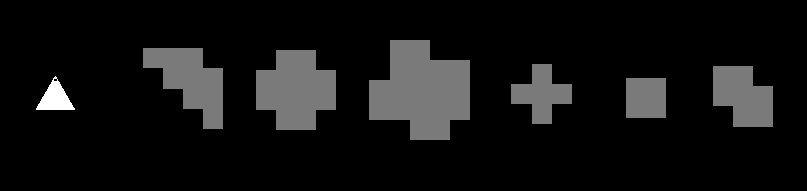
\includegraphics[width=0.5\linewidth]{agent-next-to-clusters.png}
    \parbox{0.75\textwidth}{
        \caption{Ένας πράκτορας (αριστερά) και όλες οι διαφορετικές συστάδες που μπορεί να τοποθετήσει ο αλγόριθμος.}
        \label{fig:agent-next-to-clusters}
    }
\end{figure}

\begin{figure}[H]
    \centering
    
\includegraphics[width=0.3\linewidth]{part-destroyed-cluster.png}
    \parbox{0.75\textwidth}{
        \caption{Μία συστάδα μετά που έχει δεχτεί ζημιά σε τμήματά της (αριστερά) συγκριτικά με την αρχική της κατάσταση (δεξιά).}
        \label{fig:arena_layout}
    }
\end{figure}

\begin{figure}[H]
    \centering
    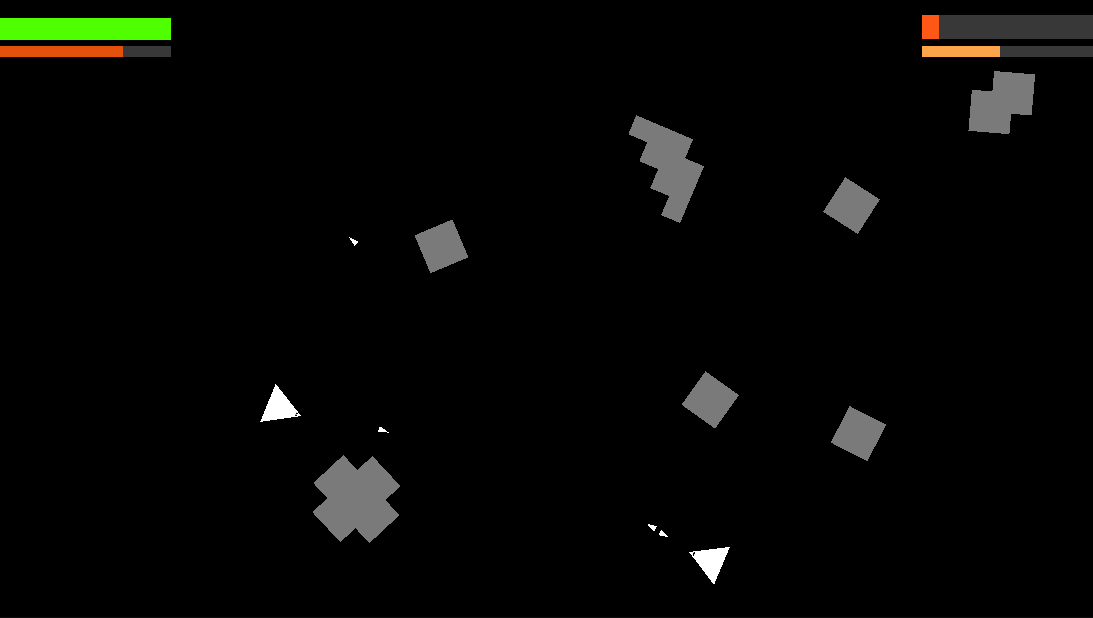
\includegraphics[width=0.5\linewidth]{in-combat-ss.png}
    \parbox{0.75\textwidth}{
        \caption{Ένα στιγμιότυπο της αρένας. Στις πάνω γωνίες φαίνονται οι πόντοι ζωής και η θερμοκρασία του κάθε πράκτορα.}
        \label{fig:in-combat-ss}
    }
\end{figure}

\begin{table}[H]
\centering
\caption{Παράμετροι Περιβάλλοντος}
\label{tab:env-params}
\begin{tabular}{ll}
\hline
\textbf{Παράμετρος} & \textbf{Τιμή} \\
\hline
Διαστάσεις αρένας & [(26.67, 15)] \\
Πόντοι ζωής πράκτορα (HP) & 100 HP \\
Ταχύτητα κίνησης & 6 m/s \\
Ρυθμός περιστροφής & 130 deg/s \\
Ζημιά βλήματος & -15 HP \\
Ταχύτητα βλήματος & 25 m/s \\
Χρόνος ζωής βλήματος & 0.7 s \\
Χρόνος αναμονής μεταξύ διαδοχικών βολών & 0.25 s \\
Αύξηση θερμοκρασίας ανά πυροβολισμό & +10 Heat \\
Ανώτατο όριο θερμοκρασίας & 50 Heat \\
Ρυθμός πτώσης θερμοκρασίας & -15 Heat/s \\
Διάρκεια ποινής υπερθέρμανσης & 3 s \\
Πόντοι ζωής τμημάτων εμποδίου & 30 HP \\
Μέγιστο πλήθος εμποδίων ανά επεισόδιο & 15 \\
Μέγιστος αριθμός δοκιμών τοποθέτησης εμποδίων & 30 \\
Πιθανότητα εναλλαγής σημείων γέννεσης & 50\% \\
\hline
\end{tabular}
\end{table}

\section{Μέθοδοι Τεχνητής Νοημοσύνης για πράκτορες παιχνιδιών}
\subsection{Πράκτορας Βασισμένος σε Κανόνες}
Ο πράκτορας βασισμένος σε κανόνες σχεδιάστηκε γύρω από δύο θεμελιώδη συστατικά:
\begin{itemize}
    \item Μία μηχανή πεπερασμένων καταστάσεων (Finite State Machine, FSM), η οποία υλοποιήθηκε χειροκίνητα, είναι υπεύθυνη για τη συμπεριφορά και την στρατηγική που ακολουθεί ο πράκτορας, (πότε επιτίθεται, πότε υποχωρεί, κ.λπ.).
    \item Τον αλγόριθμο A*, όπως παρέχεται εγγενώς από το Unity (μέσω του συστήματος NavMesh), αναλαμβάνει αποκλειστικά το υποπρόβλημα της πλοήγησης (εύρεση διαδρομής προς έναν επιθυμητό προορισμό). 
\end{itemize}
Ο διαχωρισμός αυτός επιτρέπει στην FSM να αποφασίζει τι πρέπει να κάνει ο πράκτορας σε υψηλό επίπεδο (π.χ. "πλησίασε τον αντίπαλο", "αναζήτησε κάλυψη"), αφήνοντας το πώς θα φτάσει εκεί στον A*.

\subsubsection{Βασική εκδοχή}
Η πρώτη υλοποίηση αφορά έναν βασικό πράκτορα προκαθορισμένης συμπεριφοράς, ο οποίος λειτουργεί ως σημείο αναφοράς (baseline) για τη σύγκριση με τους RL πράκτορες.

Η FSM της βασικής εκδοχής έχει τις παρακάτω καταστάσεις:
\begin{itemize}
    \item \textbf{Κατάσταση «Εντός Εμβέλειας» (In-Range):} 
    Ενεργοποιείται όταν ο αντίπαλος βρίσκεται εντός της προκαθορισμένης ακτίνας εμβέλειας. Σε αυτή την κατάσταση, ο πράκτορας περιστρέφεται ώστε να στοχεύει, με δυνατότητα απόκλισης μερικών μοιρών, τον αντίπαλο και, εφόσον δεν κινδυνεύει να υπερθερμανθεί, πυροβολάει.
    \begin{itemize}
        \item \textit{Μεταβάσεις:} Μεταβαίνει στην κατάσταση \textit{«Υπερθέρμανση»} εάν η θερμοκρασία του ξεπεράσει το ανώτατο επιτρεπτό όριο, ή στην κατάσταση \textit{«Εκτός Εμβέλειας»} εάν ο στόχος απομακρυνθεί ή δεν υπάρχει ευθεία οπτικής επαφής (line of sight).
    \end{itemize}

    \item \textbf{Κατάσταση «Εκτός Εμβέλειας» (Out-of-Range):} 
    Ενεργοποιείται όταν ο αντίπαλος βρίσκεται εκτός της προκαθορισμένης ακτίνας εμβέλειας ή δεν υπάρχει ευθεία οπτικής επαφής. Ο πράκτορας αξιοποιεί τον αλγόριθμο πλοήγησης $A^*$ για να κινηθεί προς την τοποθεσία του αντιπάλου, εκτελώντας περιστροφές, εφόσον χρειάζεται, ώστε να παραμείνει στοχευμένος.
    \begin{itemize}
        \item \textit{Μεταβάσεις:} Μεταβαίνει στην κατάσταση \textit{«Εντός Εμβέλειας»} μόλις ο αντίπαλος βρεθεί εντός εμβέλειας και εξασφαλιστεί καθαρό οπτικό πεδίο.
    \end{itemize}

    \item \textbf{Κατάσταση «Υπερθέρμανση» (Overheated):} 
    Ενεργοποιείται όταν η θερμοκρασία του πράκτορα υπερβεί ένα θερμικό όριο. Ο πράκτορας ακινητοποιείται, αλλά διατηρεί τη δυνατότητα περιστροφής ώστε να παραμένει στοχευμένος στον αντίπαλο, και αναμένει την πτώση της θερμοκρασίας του.
    \begin{itemize}
        \item \textit{Μεταβάσεις:} Μεταβαίνει στην κατάσταση \textit{«Εκτός Εμβέλειας»} μόλις η θερμοκρασία υποχωρήσει κάτω από το ασφαλές κατώφλι επαναφοράς.
    \end{itemize}
\end{itemize}

\subsubsection{Σύνθετη Εκδοχή}
Η δεύτερη υλοποίηση αφορά έναν σύνθετο πράκτορα, ο οποίος λειτουργεί ως μία δοκιμασία πιο κοντά σε πραγματικό πράκτορα παιχνιδιού.

Η FSM της σύνθετης εκδοχής έχει τις παρακάτω καταστάσεις:
\begin{itemize}
    \item \textbf{Κατάσταση «Εντός Εμβέλειας» (In-Range / Attack):} 
    Ενεργοποιείται όταν ο αντίπαλος βρίσκεται εντός της προκαθορισμένης ακτίνας εμβέλειας. Σε αυτή την κατάσταση, ο πράκτορας περιστρέφεται ώστε να στοχεύει, με δυνατότητα απόκλισης μερικών μοιρών, την προβλεπόμενη μελλοντική θέση του αντιπάλου, την οποία υπολογίζει βάσει ταχύτητας και, εφόσον δεν κινδυνεύει να υπερθερμανθεί, πυροβολάει.
    \begin{itemize}
        \item \textit{Μεταβάσεις:} Μεταβαίνει στην κατάσταση \textit{«Υπερθέρμανση»} εάν η θερμοκρασία του ξεπεράσει το ανώτατο επιτρεπτό όριο, ή στην κατάσταση \textit{«Εκτός Εμβέλειας»} εάν ο στόχος απομακρυνθεί ή δεν υπάρχει ευθεία οπτικής επαφής (line of sight).
    \end{itemize}

    \item \textbf{Κατάσταση «Εκτός Εμβέλειας» (Out-of-Range):} 
    Ενεργοποιείται όταν ο αντίπαλος βρίσκεται εκτός της προκαθορισμένης ακτίνας εμβέλειας ή δεν υπάρχει ευθεία οπτικής επαφής. Ο πράκτορας αξιοποιεί τον αλγόριθμο πλοήγησης $A^*$ για να κινηθεί προς την τοποθεσία του αντιπάλου, εκτελώντας περιστροφές, εφόσον χρειάζεται, ώστε να παραμείνει στοχευμένος στην προβλεπόμενη μελλοντική θέση του αντίπαλου.
    \begin{itemize}
        \item \textit{Μεταβάσεις:} Μεταβαίνει στην κατάσταση \textit{«Εντός Εμβέλειας»} μόλις ο αντίπαλος βρεθεί εντός εμβέλειας και εξασφαλιστεί καθαρό οπτικό πεδίο.
        Μεταβαίνει στην κατάσταση \textit{«Καταστροφή Κάλυψης»} αν ο αντίπαλος βρίσκεται εντός εμβέλειας και πίσω από αδύναμη κάλυψη.
    \end{itemize}

    \item \textbf{Κατάσταση «Καταστροφή Κάλυψης»:}
    Ενεργοποιείται όταν ο αντίπαλος βρίσκεται εκτός ευθείας οπτικής επαφής, εντός εμβέλειας και πίσω από αδύναμη κάλυψη. Αδύναμη θεωρείται η κάλυψη της οποίας το σύνολο πόντων ζωής των τμημάτων των συστάδων που την συντελούν, είναι λιγότερο από ένα κατώφλι. Ο πράκτορας πυροβολεί την αδύναμη κάλυψη χωρίς όμως να ξεπεράσει μία μέγιστη θερμοκρασία, ώστε να έχει περιθώριο να πυροβολήσει όταν αποκτήσει την ευθεία οπτικής επαφής.
    \begin{itemize}
        \item \textit{Μεταβάσεις:} Μεταβαίνει στην κατάσταση \textit{«Εντός Εμβέλειας»} μόλις εξασφαλιστεί καθαρό οπτικό πεδίο.
        Μεταβαίνει στην κατάσταση \textit{«Εκτός Εμβέλειας»} αν ο αντίπαλος κινηθεί εκτός εμβέλειας η πίσω από δυνατή (μη αδύναμη) κάλυψη.
    \end{itemize}

    \item \textbf{Κατάσταση «Υπερθέρμανση» (Overheated):} 
    Ενεργοποιείται όταν η θερμοκρασία του πράκτορα υπερβεί ένα θερμικό όριο. Ο πράκτορας επιλέγει τυχαία ένα σημείο εντός ενός διαστήματος μοιρών στην αντίθετη από τον αντίπαλο κατεύθυνση και δραπετεύει προς εκείνη την κατεύθυνση. Μετά από ένα χρονικό διάστημα επιλέγει άλλο τυχαίο σημείο διαφυγής και καθ' ολη τη διάρκεια αναμονής της πτώσης της θερμοκρασίας του, παραμένει στοχευμένος στον αντίπαλο.
    \begin{itemize}
        \item \textit{Μεταβάσεις:} Μεταβαίνει στην κατάσταση \textit{«Εκτός Εμβέλειας»} μόλις η θερμοκρασία υποχωρήσει κάτω από το ασφαλές κατώφλι επαναφοράς.
    \end{itemize}
\end{itemize}

Η εμβέλεια των πρακτόρων προκύπτει από το 75\% της μέγιστης απόστασης που διανύει μια σφαίρα.

\begin{table}[H]
\centering
\caption{Παράμετροι Σύνθετης Εκδοχής Πράκτορα Βασισμένου σε Κανόνες}
\label{tab:complex-fsm-params}
\begin{tabular}{ll}
\hline
\textbf{Παράμετρος} & \textbf{Τιμή} \\
\hline
Εμβέλεια πράκτορα & 13.125 m \\
Περιθώριο σφάλματος στόχευσης & 3 deg \\
Όριο λήξης υπερθέρμανσης & 10\% Heat \\
Όριο έναρξης υπερθέρμανσης & 85\% Heat \\
\textit{Εύρος τυχαίας γωνίας διαφυγής}$^{*}$ & $\pm$30 deg \\
\textit{Χρονικό διάστημα ανανέωσης σημείου διαφυγής}$^{*}$ & 0.3 s \\
\textit{Κατώφλι αδύναμης κάλυψης}$^{*}$ & 90 HP \\
\textit{Όριο θερμοκρασίας στη διαδικασία καταστροφής κάλυψης}$^{*}$ & 60\% Heat \\
\hline
\end{tabular}

\vspace{4pt}
\raggedright
\footnotesize{$^{*}$Παράμετρος που αφορά αποκλειστικά τη σύνθετη εκδοχή του πράκτορα.}
\end{table}

\subsection{Πράκτορας βασισμένος σε Ενισχυτική Μάθηση}
\subsubsection{Παρατηρήσεις (Observation Space)}
Ο πράκτορας RL λαμβάνει πληροφορία για την κατάσταση του περιβάλλοντος μέσω δύο καναλιών: ενός διανύσματος παρατηρήσεων (observation vector) και ενός αισθητήρα ακτίνων αντίληψης (Ray Perception Sensor), ο οποίος παρέχεται από το ML-Agents και επιτρέπει στον πράκτορα να αντιλαμβάνεται τη θέση εμποδίων, τοίχων και βολών γύρω του μέσω ακτίνων που εκτοξεύονται σε καθορισμένες γωνίες.

Το διάνυσμα παρατηρήσεων περιλαμβάνει:

\begin{itemize}
\item Το σχετικό διάνυσμα θέσης προς τον αντίπαλο (2 τιμές),
\item Τη σχετική γωνία προς τον αντίπαλο, κανονικοποιημένη στο διάστημα [−1,1] (1 τιμή),
\item Το διάνυσμα προσανατολισμού (forward direction) του ίδιου του πράκτορα (2 τιμές),
\item Το διάνυσμα προσανατολισμού του αντιπάλου (2 τιμές),
\item Το ποσοστό των πόντων ζωής του ίδιου του πράκτορα (1 τιμή),
\item Το ποσοστό τρέχουσας θερμοκρασίας του ίδιου του πράκτορα (1 τιμή),
\item Δυαδική ένδειξη κατάστασης υπερθέρμανσης του ίδιου του πράκτορα (1 τιμή),
\item Το ποσοστό των πόντων ζωής του αντιπάλου (1 τιμή),
\item Δυαδική ένδειξη δυνατότητας πυροβολισμού (δεν βρίσκεται σε αναμονή μεταξύ βολών) (1 τιμή),
\item Το διάνυσμα τρέχουσας γραμμικής ταχύτητας του πράκτορα (2 τιμές),
\end{itemize}

Για την αντίληψη της γεωμετρίας της αρένας, ο πράκτορας αξιοποιεί έναν αισθητήρα ακτίνων αντίληψης (Ray Perception Sensor), ο οποίος εκπέμπει συνολικά 16 ακτίνες, κατανεμημένες συμμετρικά εντός εύρους 360°, καλύπτοντας ουσιαστικά κάθε κατεύθυνση γύρω από τον πράκτορα. Κάθε ακτίνα ελέγχει το σημείο σύγκρουσης σε έναν κύκλο ακτίνας $0.5$, προσδίδοντας ανοχή στην ανίχνευση αντικειμένων. Ο αισθητήρας επιστρέφει, για κάθε ακτίνα, πληροφορία σχετικά με το αν και σε ποια απόσταση συναντά αντικείμενο του περιβάλλοντος τα οποία ανήκουν του συνόλου: {Εμπόδιο, Σφαίρα, Αντίπαλος} προσφέροντας στον πράκτορα την απαραίτητη πληροφόρηση για την τοπική γεωμετρία γύρω του δυναμικά, σύμφωνα με τη θέση του στον χώρο.

Οι παρατηρήσεις είναι 30 συμπεριλαμβανομένων και των παρατηρήσεων του Ray Perception Sensor.

\subsubsection{Ενέργειες (Action Space)}
Ο χώρος ενεργειών του πράκτορα RL αντιστοιχεί άμεσα στις τρεις θεμελιώδεις ενέργειες του περιβάλλοντος, όπως περιγράφηκαν στην προηγούμενη ενότητα: κίνηση, περιστροφή και πυροβολισμός. Συγκεκριμένα, υλοποιείται μέσω δύο συνεχών ενεργειών κίνησης (κατά τους άξονες x και y), μίας συνεχούς ενέργειας περιστροφής, και μίας διακριτής, δυαδικής ενέργειας πυροβολισμού (πυροβολεί/δεν πυροβολεί). Η ενέργεια του πυροβολισμού εκτελείται μόνο εφόσον ικανοποιούνται ταυτόχρονα οι συνθήκες δυνατότητας πυροβολισμού τόσο ως προς τον χρόνο αναμονής μεταξύ βολών, όσο και ως προς την κατάσταση θερμοκρασίας.

\subsubsection{Συνάρτηση Ανταμοιβής (Reward Function)}
Η συνάρτηση ανταμοιβής σχεδιάστηκε σκόπιμα αραιή (sparse), αποφεύγοντας την εκτεταμένο  ώστε ο πράκτορας να αναπτύξει στρατηγική συμπεριφορά μέσα από ελάχιστη καθοδήγηση, ενισχύοντας τη γενικευσιμότητα της μαθημένης πολιτικής. 

Συγκεκριμένα έχουν οριστεί 4 αμοιβές / ποινές:

\begin{itemize}
\item Αμοιβή +0.15 σε περίπτωση πετυχημένης βολής.
\item Ποινή -0.15 σε περίπτωση που πετύχει ο αντίπαλος βολή.
\item Αμοιβή 1 σε περίπτωση νίκης.
\item Ποινή -1 σε περίπτωση ήττας.
\end{itemize}

% TODO: Consider adding description on what each reward achieves.

\subsection{Μεθοδολογίες Εκπαίδευσης}
\subsubsection{Απλή μέθοδος εκπαίδευσης}
Στην απλούστερη μορφή της η εκπαίδευση του πράκτορα γίνεται με μονομαχίες ενάντια μίας από τις δύο εκδοχές του πράκτορα βασισμένου σε κανόνες. Ο πράκτορας μπορεί να εκπαιδευτεί σε κάθε εκδοχή ξεχωριστά ή να εκπαιδευτεί πρώτα στη βασική εκδοχή (baseline) και μετά να τη χρησιμοποιήσει ως σημείο εκκίνησης, ώστε να εκπαιδευτεί στην σύνθετη εκδοχή. Ο στόχος αυτής της λογικής είναι ο πράκτορας να μάθει να παίζει το παιχνίδι αρχικά σε ένα επιεικές περιβάλλον, και στη συνέχεια να χρησιμοποιήσει τις γνώσεις του για να προσαρμοστεί γρηγορότερα και αποτελεσματικότερα στη στρατηγική ενός εξυπνότερου αντιπάλου.

\subsubsection{Μέθοδος εκπαίδευσης Self-Play}
Δεδομένου του συμμετρικού, ανταγωνιστικού χαρακτήρα του περιβάλλοντος, η εκπαίδευση του πράκτορα RL μπορεί να πραγματοποιηθεί και μέσω self-play, μιας τεχνικής κατά την οποία ο πράκτορας εκπαιδεύεται αντιμετωπίζοντας αντίγραφα (snapshots) παλαιότερων εκδοχών της δικής του πολιτικής, αντί για έναν στατικό ή προκαθορισμένο αντίπαλο. 

Το ML-Agents Toolkit παρέχει ενσωματωμένη υποστήριξη για self-play, αποθηκεύοντας περιοδικά snapshots της τρέχουσας πολιτικής τα οποία χρησιμοποιεί στη συνέχεια ως αντιπάλους κατά τη διάρκεια της εκπαίδευσης, επιτρέποντας στον πράκτορα να αντιμετωπίζει σταδιακά ισχυρότερες εκδοχές του εαυτού του καθώς η εκπαίδευση προχωρά.

Η επιλογή του self-play, βασίστηκε τόσο σε θεωρητικούς όσο και σε πρακτικούς λόγους. Από θεωρητική σκοπιά, η εκπαίδευση εναντίον στατικού αντιπάλου διατρέχει τον κίνδυνο ο πράκτορας να προσαρμοστεί υπερβολικά (overfit) στις συγκεκριμένες αδυναμίες ή προβλέψιμα πρότυπα συμπεριφοράς εκείνου του αντιπάλου, αντί να αναπτύξει μία αποτελεσματική γενική στρατηγική. Ένας ακόμα λόγος είναι ότι, ακόμα και ο πιο απλός αντίπαλος βασισμένος σε κανόνες, αποδείχθηκε είναι πολύ δύσκολος για εκπαίδευση με αραιές αμοιβές. Από πρακτική σκοπιά, προκαταρκτικές δοκιμές εκπαίδευσης χωρίς μηχανισμό self-play οδήγησαν σε ιδιαίτερα απλοϊκές και συχνά αναποτελεσματικές πολιτικές.

\subsection{Υποδομή Εκπαίδευσης}
Η εκπαίδευση πραγματοποιήθηκε αποκλειστικά σε επεξεργαστή (CPU), δεδομένου ότι η αρχιτεκτονική δικτύου που χρησιμοποιεί το ML-Agents για προβλήματα αυτού του τύπου βασίζεται σε πλήρως συνδεδεμένα (fully-connected) στρώματα αντί για συνελικτικά νευρωνικά δίκτυα (CNN), καθιστώντας τη χρήση κάρτας γραφικών (GPU) μη απαραίτητη για σημαντική επιτάχυνση. Η εκπαίδευση πραγματοποιήθηκε με παραλληλισμό σε 8 παράλληλα περιβάλλοντα εκπαίδευσης που συλλέγουν τροχιές, σε έναν επεξεργαστή με 6 φυσικούς πυρήνες και ταχύτητα ρολογιού ~4.5 GHz. (\foreignlanguage{english}{Ryzen 5 7600X})

\section{Πειραματική αξιολόγηση}
\subsection{PPO εναντίον Απλής Εκδοχής}
\subsubsection{Κύριες Παράμετροι Πειράματος}
Η διαμόρφωση των υπερπαραμέτρων του PPO που χρησιμοποιήθηκε στις υποενότητες 5.1 και 5.2 παρουσιάζεται στον Πίνακα 3. Οι τιμές επιλέχθηκαν βάσει καθιερωμένων προεπιλογών του ML-Agents Toolkit, με στοχευμένες προσαρμογές ώστε να ταιριάζουν στο μέγεθος του χώρου παρατηρήσεων. 

Συγκεκριμένα, ο ρυθμός μάθησης (\foreignlanguage{english}{learning rate}) ορίστηκε στο $3 \cdot 10^{-4}$, μια ευρέως χρησιμοποιούμενη τιμή για τον αλγόριθμο \foreignlanguage{english}{PPO} που εξισορροπεί την ταχύτητα σύγκλισης και τη σταθερότητα της εκπαίδευσης. Το μέγεθος του δικτύου πολιτικής (\foreignlanguage{english}{policy network}) ορίστηκε σε δύο κρυφά στρώματα (\foreignlanguage{english}{hidden layers}) των 256 νευρώνων, μέγεθος επαρκές για τον σχετικά περιορισμένο χώρο παρατηρήσεων (\foreignlanguage{english}{observation space}), χωρίς να επιβαρύνει υπερβολικά τον χρόνο εκπαίδευσης. Τέλος, χρησιμοποιήθηκε πρόσθετο σήμα εσωτερικής ανταμοιβής «περιέργειας» (\foreignlanguage{english}{curiosity reward signal}), με σχετικά χαμηλή ένταση (\foreignlanguage{english}{strength} $0.02$) ως προς το κύριο εξωτερικό σήμα ανταμοιβής (\foreignlanguage{english}{strength} $1.0$), με στόχο την ενίσχυση της εξερεύνησης (\foreignlanguage{english}{exploration}) του πράκτορα, δεδομένης της αραιής (\foreignlanguage{english}{sparse}) φύσης της συνάρτησης ανταμοιβής. Η περιέργεια προσφέρει μια μικρή επιβράβευση στον πράκτορα όταν μεταβαίνει σε καταστάσεις με υψηλή αβεβαιότητα πρόβλεψης, αποτελώντας έτσι ένα χρήσιμο εργαλείο για την αποφυγή εγκλωβισμού σε τοπικά βέλτιστα (\foreignlanguage{english}{local optima}).

\begin{table}[H]
\centering
\caption{Διαμόρφωση Υπερπαραμέτρων PPO}
\label{tab:ppo-config}
\begin{tabular}{ll}
\hline
\textbf{Υπερπαράμετρος} & \textbf{Τιμή} \\
\hline
Batch size & 512 \\
Buffer size & 16384 \\
Learning rate & $3 \cdot 10^{−4}$ (linear schedule) \\
Epsilon (clip) & 0.2 (linear schedule) \\
Beta (entropy coefficient) & 0.01 (constant) \\
Number of epochs & 3 \\
Hidden units & 256 \\
Number of layers & 2 \\
Gamma (discount factor) & 0.99 \\
Extrinsic reward strength & 1.0 \\
Curiosity reward strength & 0.02 \\
Time horizon & 256 \\
\hline
\end{tabular}
\end{table}

\subsubsection{Αποτελέσματα Πειράματος με 5 εκατομμύρια βήματα}
Ο πράκτορας παρουσίασε σαφή και σταθερή σύγκλιση καθ' όλη τη διάρκεια της εκπαίδευσης. Το ποσοστό νικών (Win Rate) αυξήθηκε σταδιακά από μηδενικές τιμές στην αρχή της εκπαίδευσης σε περίπου 55\% κατά τη λήξη της, υποδεικνύοντας ότι ο πράκτορας κατάφερε να αναπτύξει μία μερικώς αποδοτική στρατηγική εναντίον του συγκεκριμένου αντιπάλου. Αντίστοιχα, η αθροιστική ανταμοιβή (Cumulative Reward) παρουσίασε ομαλή, μονότονη αύξηση, χωρίς σημάδια αστάθειας ή απότομων πτώσεων απόδοσης.

Η ποιοτική εξέταση της συμπεριφοράς του αποκαλύπτει σαφή ασυμμετρία μεταξύ άμυνας και επίθεσης. Ο πράκτορας πυροβολεί με πολύ υψηλή συχνότητα και ασθενή ένδειξη στοχευμένης προσπάθειας, γεγονός το οποίο επιβεβαιώνεται και από τη χαμηλή ακρίβεια των βολών του (~10\%–13\%), την σχετικά υψηλή μέση θερμοκρασία (~56\%) και τον υψηλό αριθμό βολών ανά γύρο (~45). Οι περιστροφές του πράκτορα παραμένουν σε μεγάλο βαθμό τυχαίες, εμφανιζόμενες ακόμη και σε στιγμές όπου δεν φαίνεται να εξυπηρετούν άμεσο σκοπό στοχοθεσίας. Ωστόσο, το ποσοστό αποτελεσματικής αποφυγής βλημάτων του αντιπάλου έφτασε περίπου στο 90\%, υποδεικνύοντας ότι ο πράκτορας ανέπτυξε ιδιαίτερα αποτελεσματική αμυντική/αποφευκτική συμπεριφορά, σημαντικά ισχυρότερη από την επιθετική του ικανότητα.

Η οριακά θετική αναλογία νίκης επιτυγχάνεται, επομένως, λόγω της αποτελεσματικής άμυνας, η συνεχή κίνηση καθιστά την στρατηγική του αντιπάλου του μη αποτελεσματική και, παρά την χαμηλή ευστοχία του, τελικά νικάει. Η συμπεριφορά αυτή αναδεικνύει μια ενδιαφέρουσα πτυχή της αραιής συνάρτησης ανταμοιβής που χρησιμοποιήθηκε: ο πράκτορας εντόπισε μια στρατηγική που εξασφαλίζει ικανοποιητικό, αλλά όχι βέλτιστο, ποσοστό νικών, χωρίς ωστόσο να αναπτύξει την πιο εκλεπτυσμένη, στοχευμένη επιθετική συμπεριφορά που θα αναμενόταν από έναν πλήρως εκπαιδευμένο πράκτορα.

\subsubsection{Αποτελέσματα Πειράματος με 10 εκατομμύρια βήματα}
Ο πράκτορας PPO εκπαιδεύτηκε εναντίον της απλής εκδοχής του πράκτορα βασισμένου σε κανόνες για συνολικά 10 εκατομμύρια βήματα, διπλάσια διάρκεια από το αρχικό πειραματικό σχέδιο, προκειμένου να εξεταστεί κατά πόσο η παρατηρούμενη συμπεριφορά αποτελούσε μεταβατικό στάδιο ή σταθεροποιημένη πολιτική. Τα αποτελέσματα δείχνουν ότι το ποσοστό νικών συνέχισε να βελτιώνεται, φτάνοντας τελικά περίπου στο 87\%–88\%, έναντι του 50\%–55\%. Αντίστοιχη βελτίωση παρατηρείται και στην αθροιστική ανταμοιβή, η οποία συνέχισε την ανοδική της πορεία χωρίς ενδείξεις σταθεροποίησης μέχρι και το τέλος της εκπαίδευσης.

Η ανάλυση των επιμέρους μετρικών αποκαλύπτει ότι η επιπλέον εκπαίδευση οδήγησε σε ποσοτική βελτίωση της ίδιας βασικής τακτικής, όχι στην ανάδυση μιας ποιοτικά διαφορετικής στρατηγικής. Η ακρίβεια πυροβολισμού αυξήθηκε από περίπου 13\% στα 5M σε περίπου 22\% στα 10M βήματα, ενώ ο μέσος αριθμός βολών ανά γύρο, υποχώρησε σταθερά σε περίπου 33 βολές ανά γύρο στο τέλος της εκπαίδευσης. Η ακρίβεια του αντιπάλου εναντίον του πράκτορα μειώθηκε από περίπου 15\% σε 10\% και η μέση διάρκεια ενός γύρου όπου ο RL πράκτορας νικάει, μειώθηκε κατά 10 δευτερόλεπτα.

Παρά τις βελτιώσεις αυτές, η θεμελιώδης στρατηγική του πράκτορα παραμένει ουσιαστικά ταυτόσημη με εκείνη που παρατηρήθηκε στην εκπαίδευση των 5 εκατομμυρίων βημάτων: ο πράκτορας συνεχίζει να βασίζεται στον συνδυασμό υψηλού όγκου πυρών και ιδιαίτερα αποτελεσματικών ελιγμών αποφυγής, αντί να αναπτύσσει μια ουσιωδώς βελτιωμένη ικανότητα στόχευσης. Ειδικότερα, η πολιτική του προκρίνει συχνά τη χωρική επανατοποθέτηση (repositioning) έναντι της ενεργής περιστροφής/στόχευσης. Ο πράκτορας επιλέγει να ελίσσεται περιμετρικά και προς το μέρος του αντιπάλου, ευθυγραμμίζοντάς τον «παθητικά» στο πεδίο βολής του αποκλειστικά μέσω της μετατοπιστικής του κίνησης.

Το εύρημα αυτό ενισχύει την ερμηνεία ότι η αρχικά παρατηρούμενη συμπεριφορά αντιστοιχεί σε ένα σχετικά σταθερό τοπικό βέλτιστο (local optimum) της αραιής συνάρτησης ανταμοιβής, το οποίο η επιπλέον υπολογιστική προσπάθεια βελτιστοποιεί περαιτέρω αντί να το ξεπερνά ποιοτικά.

\subsubsection{Γραφήματα Αποτελεσμάτων}
Στα παρακάτω γραφήματα με πράσινο συμβολίζεται το πείραμα των 5 εκατομμυρίων βημάτων, ενώ με ροζ το πείραμα των 10 εκατομμυρίων βημάτων.

% 1. Γενική Απόδοση Εκπαίδευσης (Πείραμα 1)
\begin{figure}[htbp]
    \centering
    \begin{minipage}[b]{0.48\textwidth}
        \centering
        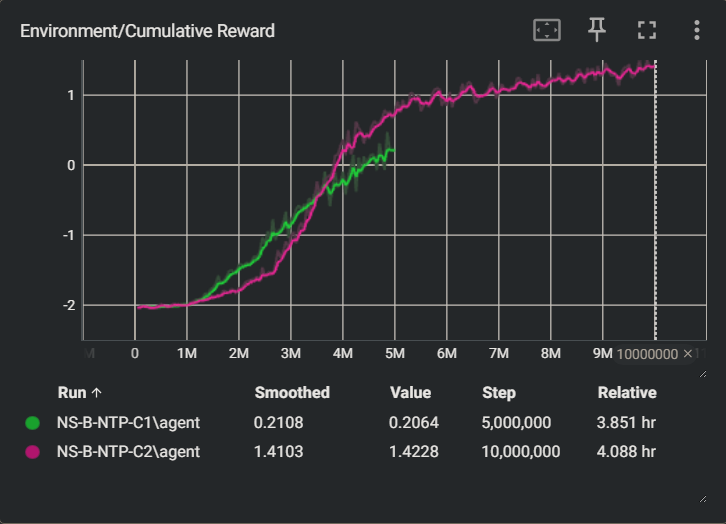
\includegraphics[width=\textwidth]{bc1-bc2-cumulative-reward.png}
        \caption{Αθροιστική ανταμοιβή (Πείραμα 1)}
        \label{fig:exp1_cumulative_reward}
    \end{minipage}
    \hfill
    \begin{minipage}[b]{0.48\textwidth}
        \centering
        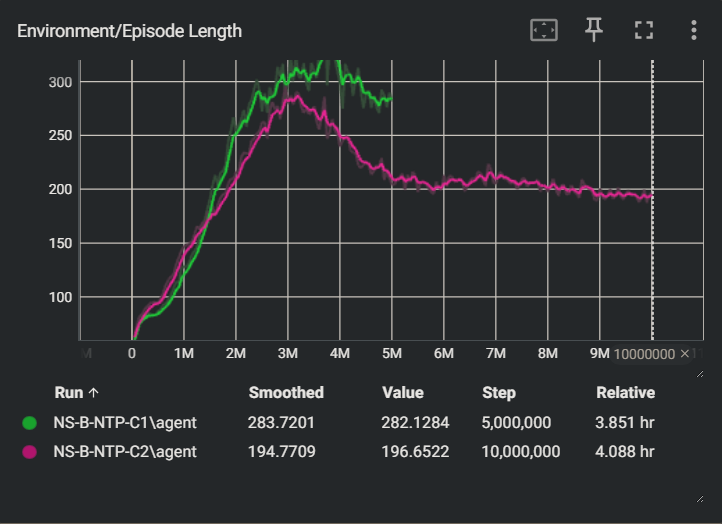
\includegraphics[width=\textwidth]{bc1-bc2-ep-length.png}
        \caption{Διάρκεια επεισοδίου (Πείραμα 1)}
        \label{fig:exp1_episode_length}
    \end{minipage}
\end{figure}

% 2. Στρατηγική Πυρομαχικών & Θερμοκρασίας (Πείραμα 1)
\begin{figure}[htbp]
    \centering
    \begin{minipage}[b]{0.48\textwidth}
        \centering
        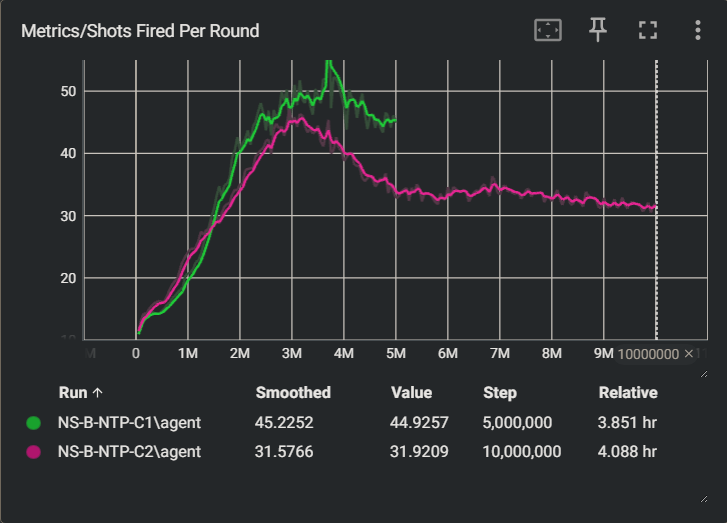
\includegraphics[width=\textwidth]{bc1-bc2-shots-per-round.png}
        \caption{Βολές ανά γύρο (Πείραμα 1)}
        \label{fig:exp1_shots_per_round}
    \end{minipage}
    \hfill
    \begin{minipage}[b]{0.48\textwidth}
        \centering
        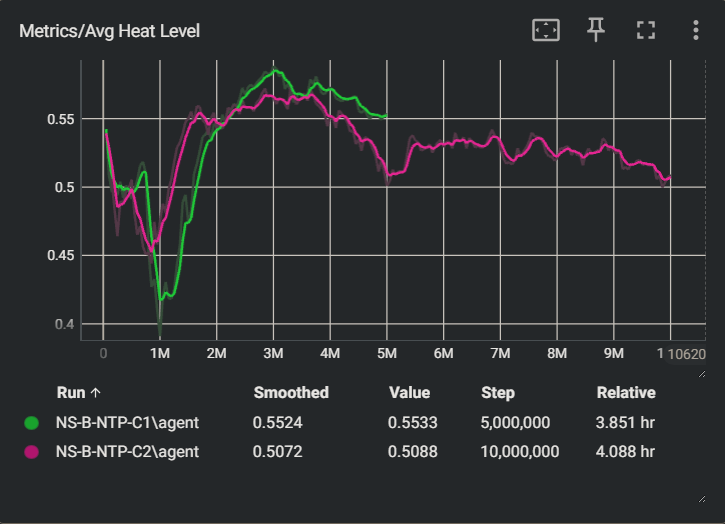
\includegraphics[width=\textwidth]{bc1-bc2-avg-heat.png}
        \caption{Μέση θερμοκρασία πράκτορα (Πείραμα 1)}
        \label{fig:exp1_avg_heat}
    \end{minipage}
\end{figure}

% 3. Σύγκριση Ακρίβειας (Πείραμα 1)
\begin{figure}[htbp]
    \centering
    \begin{minipage}[b]{0.48\textwidth}
        \centering
        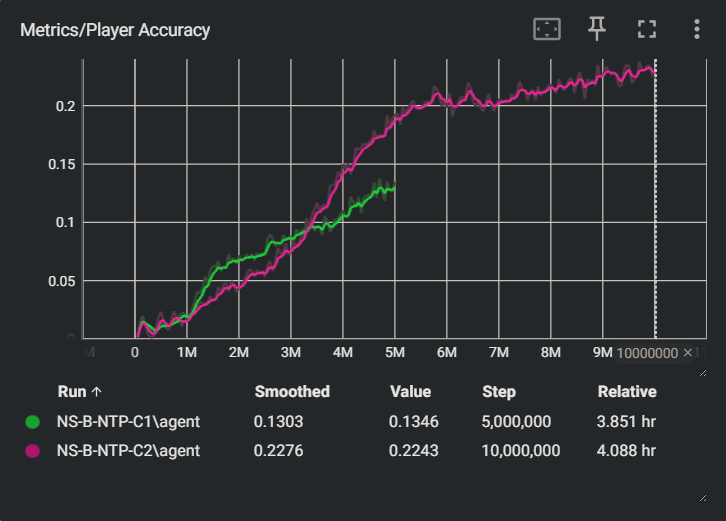
\includegraphics[width=\textwidth]{bc1-bc2-player-acc.png}
        \caption{Ακρίβεια βολών πράκτορα (Πείραμα 1)}
        \label{fig:exp1_player_acc}
    \end{minipage}
    \hfill
    \begin{minipage}[b]{0.48\textwidth}
        \centering
        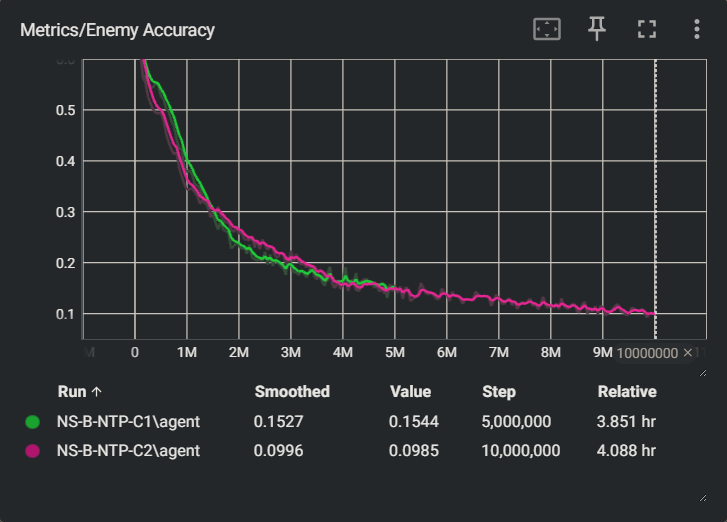
\includegraphics[width=\textwidth]{bc1-bc2-enemy-acc.png}
        \caption{Ακρίβεια βολών αντιπάλου (Πείραμα 1)}
        \label{fig:exp1_enemy_acc}
    \end{minipage}
\end{figure}

% 4. Αποτελεσματικότητα & Ποσοστό Νικών (Πείραμα 1)
\begin{figure}[htbp]
    \centering
    \begin{minipage}[b]{0.48\textwidth}
        \centering
        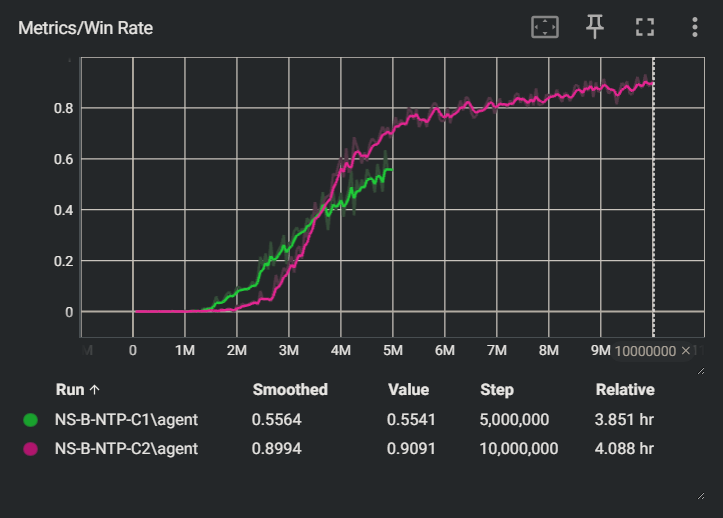
\includegraphics[width=\textwidth]{bc1-bc2-winrate.png}
        \caption{Αναλογία νίκης πράκτορα (Πείραμα 1)}
        \label{fig:exp1_winrate}
    \end{minipage}
    \hfill
    \begin{minipage}[b]{0.48\textwidth}
        \centering
        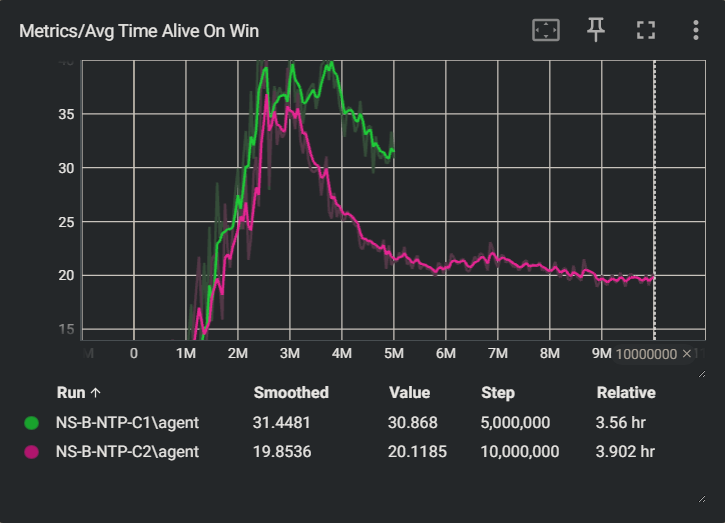
\includegraphics[width=\textwidth]{bc1-bc2-avg-dur-on-win.png}
        \caption{Διάρκεια επεισοδίου σε νίκη πράκτορα (Πείραμα 1)}
        \label{fig:exp1_avg_dur_on_win}
    \end{minipage}
\end{figure}
\begin{figure}
    \centering
    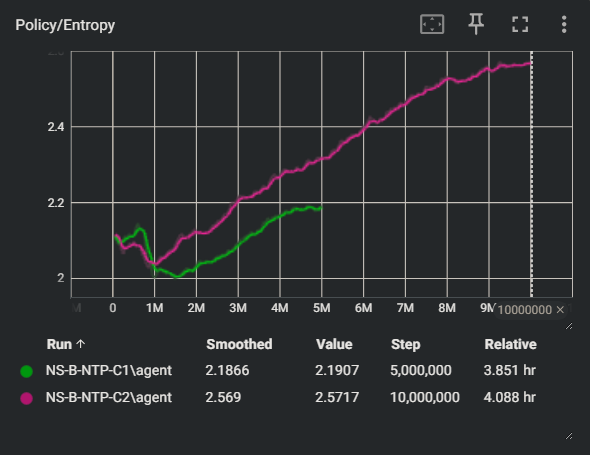
\includegraphics[width=0.48\linewidth]{bc1-bc2-entropy.png}
    \caption{Εντροπία πολιτικής (Πείραμα 1)}
    \label{fig:bc1-bc2-entropy}
\end{figure}

% ΣΥΝΘΕΤΗ ΕΚΔΟΧΗ
\subsection{PPO εναντίον Σύνθετης Εκδοχής}
\subsubsection{Κύριες Παράμετροι Πειράματος}
Το παρόν πείραμα χρησιμοποίησε την ίδια διαμόρφωση υπερπαραμέτρων PPO με αυτή της απλής εκδοχής που περιγράφτηκε στην προηγούμενη ενότητα (Πίνακας 3), με τη μοναδική διαφορά ότι η εκπαίδευση πραγματοποιήθηκε απευθείας για 10 εκατομμύρια βήματα, χωρίς ενδιάμεση σύγκριση στα 5 εκατομμύρια. Η επιλογή αυτή βασίστηκε στο εύρημα της προηγούμενης ενότητας, όπου η σύγκριση μεταξύ 5 και 10 εκατομμυρίων βημάτων εναντίον της απλής εκδοχής έδειξε ότι, σε μεγάλο βαθμό, η επιπλέον εκπαίδευση οδηγεί σε ποσοτική βελτίωση της ίδιας βασικής στρατηγικής, χωρίς ουσιώδη ποιοτική μεταβολή της συμπεριφοράς του πράκτορα. Κρίθηκε επομένως πιο αποδοτική η άμεση εκπαίδευση για 10 εκατομμύρια βήματα, ώστε το αποτέλεσμα να αντικατοπτρίζει μια ήδη σχετικά σταθεροποιημένη πολιτική.

\subsubsection{Αποτελέσματα Πειράματος με 10 εκατομμύρια βήματα}
Ο πράκτορας παρουσίασε εξαιρετικά υψηλή τελική απόδοση, με ποσοστό νικών 95\% στο τέλος της εκπαίδευσης, αισθητά υψηλότερο από το αντίστοιχο ~87\% που παρατηρήθηκε εναντίον της απλής εκδοχής υπό το ίδιο πλήθος βημάτων. Παράλληλα, η ακρίβεια πυροβολισμού βελτιώθηκε σε περίπου 37\%, σχεδόν διπλάσια της αντίστοιχης τιμής εναντίον της απλής εκδοχής, ενώ ο μέσος αριθμός βολών ανά γύρο υποχώρησε σε περίπου 17, αισθητά χαμηλότερος. Η συνδυασμένη αυτή εικόνα υψηλότερης ακρίβειας, λιγότερων βολών και υψηλότερου ποσοστού νικών υποδεικνύει ότι ο πράκτορας ανέπτυξε συγκριτικά πιο αποδοτική επιθετική συμπεριφορά εναντίον του πιο απαιτητικού αντιπάλου, παρά τη διαισθητική προσδοκία ότι ένας δυσκολότερος αντίπαλος θα οδηγούσε σε χειρότερη, όχι καλύτερη, μαθημένη πολιτική.

Η ποιοτική εξέταση της συμπεριφοράς αποσαφηνίζει τον μηχανισμό πίσω από αυτή τη βελτίωση, αναδεικνύοντας παράλληλα σημαντική συνέχεια με το πρότυπο που παρατηρήθηκε εναντίον της απλής εκδοχής. Όπως και ενάντιας της απλής εκδοχής, ο πράκτορας δεν φαίνεται να αναπτύσσει ενεργή, στοχευμένη περιστροφή προς τον αντίπαλο και βασίζεται πρωτίστως σε κατάλληλη τοποθέτηση ώστε ο αντίπαλος να βρίσκεται ήδη εντός της κατεύθυνσης πυρός του, ελαχιστοποιώντας την ανάγκη για μεγάλες προσαρμογές του στόχου. Η βελτιωμένη ακρίβεια δεν προκύπτει, επομένως, από πιο εκλεπτυσμένη στόχευση αυτή καθαυτή, αλλά από αποδοτικότερη διαχείριση της σχετικής θέσης.

Παρά την εισαγωγή τυχαίας εναλλαγής των αρχικών θέσεων (spawn points) στις δύο πλευρές της αρένας με στόχο την εξάλειψη της χωρικής προκατάληψης (positional bias), παρατηρήθηκε μια συστηματική συμπεριφορική ασυμμετρία. 'Οταν ο πράκτορας εκκινεί από τη δεξιά πλευρά, υιοθετεί την αναμενόμενη τακτική άμεσης προσέγγισης του αντιπάλου. Αντιθέτως, κατά την εκκίνηση από την αριστερή πλευρά, αποφεύγει την άμεση περιστροφή και στόχευση. Αντί αυτής, εκτελεί ελιγμούς επανατοποθέτησης με προφανή στόχο την αντιστροφή της σχετικής διάταξης, ώστε να επαναφέρει τον αντίπαλο στα αριστερά του πριν εμπλακεί σε μάχη. Η συμπεριφορά αυτή, η οποία είχε παρατηρηθεί με μειωμένη ένταση και στο προηγούμενο πείραμα, υποδηλώνει εγκλωβισμό σε μια χωρικά εξαρτημένη υποβέλτιστη πολιτική (spatially overfitted policy), η οποία επιβαρύνει τον πράκτορα με τακτικό μειονέκτημα.

\subsubsection{Γραφήματα Αποτελεσμάτων}

% 1. Γενική Απόδοση Εκπαίδευσης (Πείραμα 2)
\begin{figure}[htbp]
    \centering
    \begin{minipage}[b]{0.48\textwidth}
        \centering
        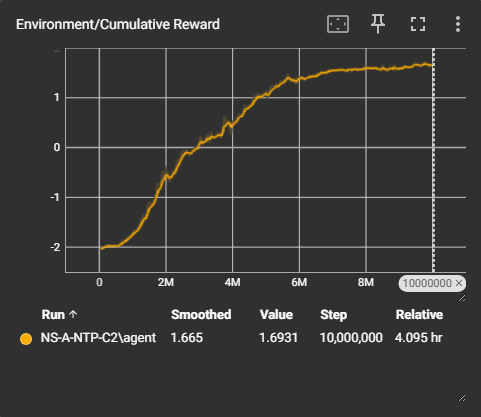
\includegraphics[width=\textwidth]{ac2-cumulative-reward.png}
        \caption{Αθροιστική ανταμοιβή (Πείραμα 2)}
        \label{fig:ac2-cumulative-reward}
    \end{minipage}
    \hfill
    \begin{minipage}[b]{0.48\textwidth}
        \centering
        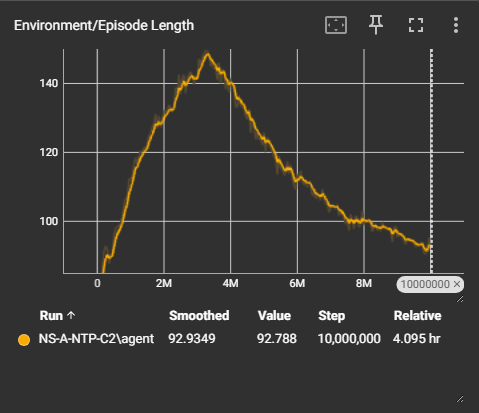
\includegraphics[width=\textwidth]{ac2-ep-length.png}
        \caption{Διάρκεια επεισοδίου (Πείραμα 2)}
        \label{fig:ac2-ep-length}
    \end{minipage}
\end{figure}

% 2. Στρατηγική Πυρομαχικών & Θερμοκρασίας (Πείραμα 2)
\begin{figure}[htbp]
    \centering
    \begin{minipage}[b]{0.48\textwidth}
        \centering
        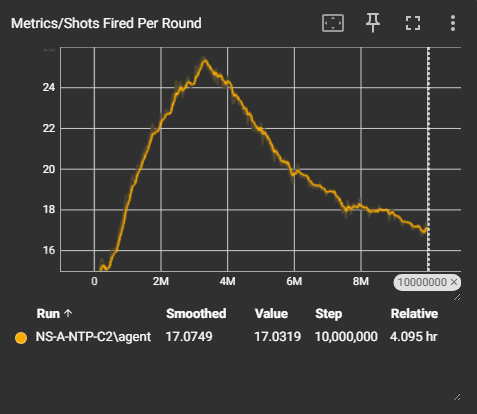
\includegraphics[width=\textwidth]{ac2-shots-fired.png}
        \caption{Βολές ανά γύρο (Πείραμα 2)}
        \label{fig:ac2-shots-fired}
    \end{minipage}
    \hfill
    \begin{minipage}[b]{0.48\textwidth}
        \centering
        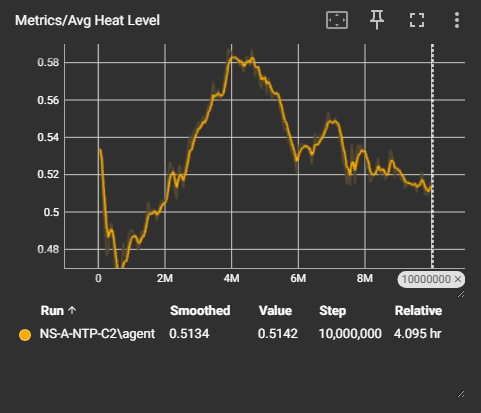
\includegraphics[width=\textwidth]{ac2-avg-heat.png}
        \caption{Μέση θερμοκρασία πράκτορα (Πείραμα 2)}
        \label{fig:ac2-avg-heat}
    \end{minipage}
\end{figure}

% 3. Σύγκριση Ακρίβειας (Πείραμα 2)
\begin{figure}[htbp]
    \centering
    \begin{minipage}[b]{0.48\textwidth}
        \centering
        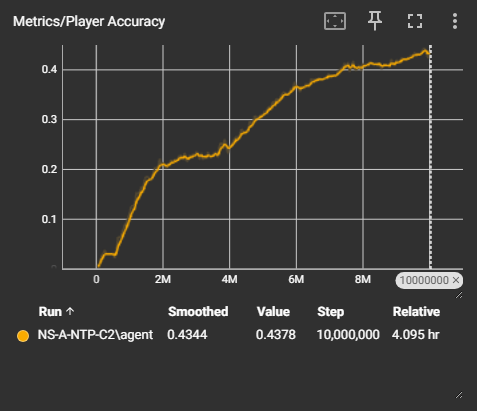
\includegraphics[width=\textwidth]{ac2-player-acc.png}
        \caption{Ακρίβεια βολών πράκτορα (Πείραμα 2)}
        \label{fig:ac2-player-acc}
    \end{minipage}
    \hfill
    \begin{minipage}[b]{0.48\textwidth}
        \centering
        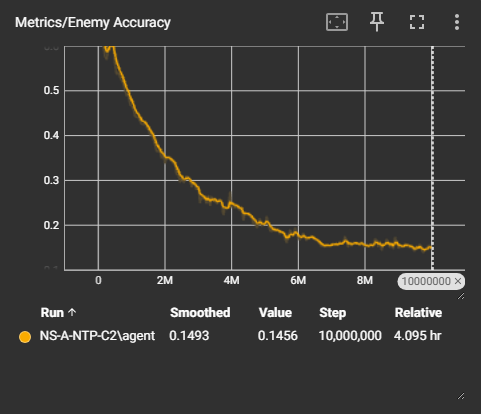
\includegraphics[width=\textwidth]{ac2-enemy-acc.png}
        \caption{Ακρίβεια βολών αντιπάλου (Πείραμα 2)}
        \label{fig:ac2-enemy-acc}
    \end{minipage}
\end{figure}
% 4. Αποτελεσματικότητα & Ποσοστό Νικών (Πείραμα 2)
\begin{figure}[htbp]
    \centering
    \begin{minipage}[b]{0.48\textwidth}
        \centering
        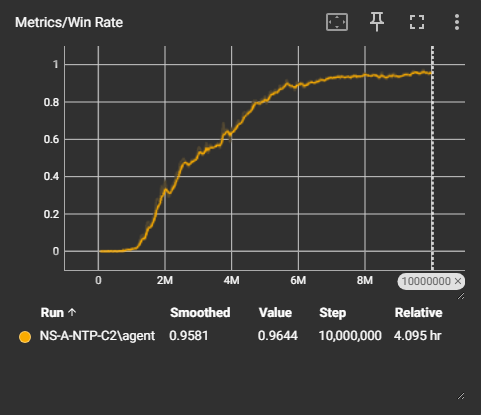
\includegraphics[width=\textwidth]{ac2-winrate.png}
        \caption{Αναλογία νίκης πράκτορα (Πείραμα 2)}
        \label{fig:ac2-winrate}
    \end{minipage}
    \hfill
    \begin{minipage}[b]{0.48\textwidth}
        \centering
        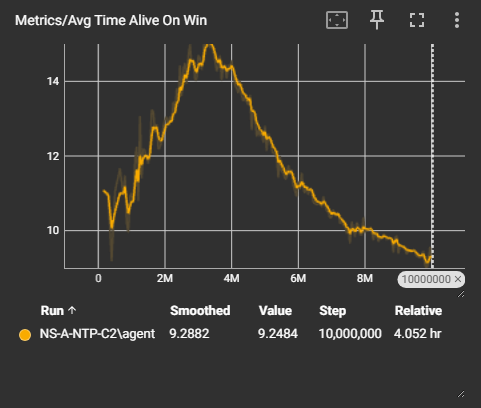
\includegraphics[width=\textwidth]{ac2-avg-dur-on-win.png}
        \caption{Διάρκεια επεισοδίου σε νίκη πράκτορα (Πείραμα 2)}
        \label{fig:ac2-avg-dur-on-win}
    \end{minipage}
\end{figure}
\begin{figure}
    \centering
    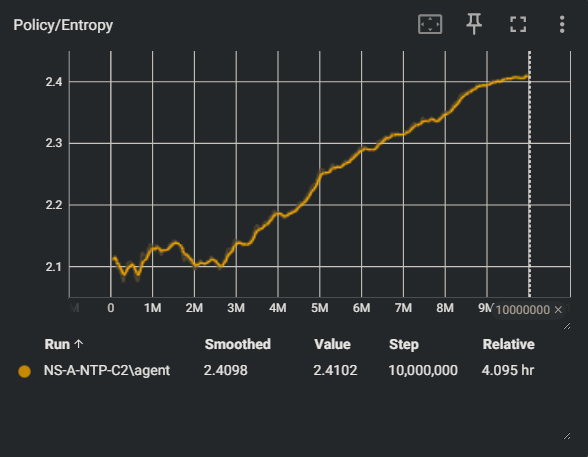
\includegraphics[width=0.5\linewidth]{ac2-entropy.png}
    \caption{Εντροπία πολιτικής (Πείραμα 2)}
    \label{fig:ac2-entropy}
\end{figure}

\subsection{PPO με Αυτό-Εκπαίδευση (Self - Play)}
\subsubsection{Κύριες Παράμετροι Πειράματος}
Η διαμόρφωση PPO που χρησιμοποιήθηκε για την εκπαίδευση self-play διαφοροποιείται σε δύο βασικά σημεία από αυτή των προηγούμενων πειραμάτων. Πρώτον, απενεργοποιήθηκε το σήμα εσωτερικής ανταμοιβής περιέργειας (curiosity), καθώς η εγγενής μη στατικότητα του αντιπάλου παρέχει ήδη σημαντική ποικιλομορφία εμπειριών, μειώνοντας την ανάγκη για πρόσθετο, τεχνητό κίνητρο εξερεύνησης, το οποίο θα μπορούσε επιπλέον να αποσπάσει την πολιτική από την αποτελεσματική προσαρμογή σε έναν ήδη διαρκώς μεταβαλλόμενο στόχο. Δεύτερον, το μέγεθος του δικτύου πολιτικής αυξήθηκε σε 512 κρυφές μονάδες κατανεμημένες σε 3 στρώματα, σε σχέση με το μικρότερο δίκτυο (256×2) που χρησιμοποιήθηκε στα πειράματα εναντίον στατικού αντιπάλου. Η αύξηση αυτή κρίθηκε σκόπιμη δεδομένου ότι η πολιτική καλείται να μάθει να αντιμετωπίζει αποτελεσματικά όχι έναν, αλλά ένα ευρύ και συνεχώς εξελισσόμενο φάσμα στρατηγικών (στιγμιότυπα του self-play), γεγονός που αυξάνει ουσιωδώς την πολυπλοκότητα του προβλήματος σε σχέση με την εκμάθηση απόκρισης σε έναν και μόνο, στατικό αντίπαλο. Το μεγαλύτερο δίκτυο παρέχει επαρκέστερη χωρητικότητα αναπαράστασης για αυτή την πιο απαιτητική, μη στατική συνθήκη μάθησης.

Ο μηχανισμός self-play ρυθμίστηκε ώστε ο πράκτορας να αντιμετωπίζει κάθε αντίπαλο (στιγμιότυπο πολιτικής) για διάστημα 10.000 βημάτων πριν αντικατασταθεί από άλλο, επιλεγμένο είτε ως το πιο πρόσφατο στιγμιότυπο (με 50\% πιθανότητα), είτε τυχαία από μια δεξαμενή έως 10 παλαιότερων στιγμιότυπων, τα οποία ανανεώνονται κάθε 40.000 βήματα. Η ισορροπία αυτή διασφαλίζει επαρκή χρόνο προσαρμογής σε κάθε συγκεκριμένο αντίπαλο πριν την εναλλαγή, ενώ παράλληλα εκθέτει τον πράκτορα τόσο στην πιο πρόσφατη όσο και σε παλαιότερες εκδοχές της πολιτικής του, αποτρέποντας την υπερβολική εξειδίκευση σε μία και μόνο, τρέχουσα στρατηγική. Η αρχική βαθμολογία ELO και των δύο πλευρών ορίστηκε στην προεπιλεγμένη τιμή 1200, ενώ ο μηχανισμός εναλλαγής ομάδας (team change) δεν χρησιμοποιήθηκε, καθώς η εναλλαγή πλευράς διασφαλίστηκε ήδη μέσω της τυχαιοποίησης των σημείων εκκίνησης στο ίδιο το περιβάλλον.

\begin{table}[H]
\centering
\caption{Διαμόρφωση Υπερπαραμέτρων Self-Play}
\label{tab:self-play-params}
\begin{tabular}{ll}
\hline
\textbf{Υπερπαράμετρος} & \textbf{Τιμή} \\
\hline
Save steps & 40000 \\
Swap steps & 10000 \\
Window & 10 \\
Play Against Latest Rate & 50\% \\
Initial ELO & 1200 \\
Learning rate & $3 \cdot 10^{−4}$ (linear schedule) \\
Epsilon (clip) & 0.2 (linear schedule) \\
Beta (entropy coefficient) & 0.01 (linear schedule) \\
Number of epochs & 3 \\
Hidden units & 512 \\
Number of hidden layers & 3 \\
Gamma (discount factor) & 0.995 \\
Time horizon & 128 \\
\hline
\end{tabular}
\end{table}

\subsubsection{Αποτελέσματα Πειράματος με 10 εκατομμύρια βήματα}
Σε αντίθεση με τα πειράματα εναντίον στατικού αντιπάλου, όπου οι βασικές μετρικές (Win Rate, Cumulative Reward, Player Accuracy) παρουσίαζαν σαφή, μονότονη ανοδική τάση μέχρι τη σταθεροποίησή τους, στο παρόν πείραμα οι αντίστοιχες μετρικές παρουσιάζουν έντονη ταλάντωση (oscillation) γύρω από μια σχετικά σταθερή τιμή, χωρίς ξεκάθαρη τάση βελτίωσης ή επιδείνωσης στην πάροδο του χρόνου. Συγκεκριμένα, το ποσοστό νικών (Win Rate) ταλαντεύεται καθ' όλη τη διάρκεια της εκπαίδευσης γύρω από το 50\% (περίπου 45\%–65\%), η αθροιστική ανταμοιβή ταλαντεύεται γύρω από το μηδέν, ενώ η ακρίβεια πυροβολισμού του πράκτορα και η αντίστοιχη ακρίβεια του αντιπάλου κινούνται σε παρόμοια, χαμηλή κλίμακα (περίπου 4\%–8\%) και με παρόμοιο εύρος διακύμανσης μεταξύ τους.

Οι διακυμάνσεις αυτές αποτελούν αναμενόμενο και, στην πραγματικότητα, επιθυμητό χαρακτηριστικό της εκπαίδευσης μέσω self-play σε ένα πλήρως συμμετρικό περιβάλλον. Επειδή ο πράκτορας εκπαιδεύεται αντιμετωπίζοντας εκδοχές του εαυτού του, οποιαδήποτε βελτίωση στην επιθετική ή αμυντική του ικανότητα αντικατοπτρίζεται ταυτόχρονα και στον αντίπαλο (αφού πρόκειται, ουσιαστικά, για την ίδια πολιτική ή πρόσφατη παραλλαγή της), με αποτέλεσμα το σχετικό πλεονέκτημα μεταξύ των δύο πλευρών να παραμένει, κατά μέσο όρο, σταθερό γύρω από την ισορροπία, ακόμη και όταν η απόλυτη ικανότητα και των δύο πλευρών αυξάνεται με την πάροδο του χρόνου. Η αδυναμία απεικόνισης αυτής της απόλυτης προόδου μέσω μετρικών όπως η αναλογία νίκης ή η αθροιστική ανταμοιβή είναι μια πρόκληση της αξιολόγησης πρακτόρων που εκπαιδεύονται μέσω self-play.

Επιπρόσθετη επιβεβαίωση παρέχει η τάση της εντροπίας, η οποία, σε αντίθεση με τα προηγούμενα πειράματα όπου παρουσίαζε αρχική πτώση πριν σταθεροποιηθεί, εδώ αυξάνεται σταθερά καθ' όλη τη διάρκεια της εκπαίδευσης. Η συνεχής αυτή αύξηση της εντροπίας υποδεικνύει ότι η πολιτική δεν συγκλίνει προς μια στατική, ντετερμινιστική συμπεριφορά, αλλά διατηρεί διαρκώς αυξανόμενο βαθμό διερευνητικότητας. Το φαινόμενο αυτό είναι απόλυτα συνεπές με ένα δυναμικό περιβάλλον όπου ο αντίπαλος εξελίσσεται παράλληλα, δημιουργώντας συνθήκες οι οποίες εμποδίζουν την πολιτική από το να προσαρμοστεί πλήρως σε μια σταθερή και εκμεταλλεύσιμη στρατηγική.

Παράλληλα, η βαθμολογία ELO παρέμεινε σταθερή στην αρχική της τιμή καθ' όλη τη διάρκεια της εκπαίδευσης. Η συμπεριφορά αυτή είναι αναμενόμενη λόγω της φύσης του self-play μηχανισμού. Καθώς ο πράκτορας αντιμετωπίζει αποκλειστικά στιγμιότυπα (snapshots) της δικής του πολιτικής, οι δύο πλευρές έχουν πολύ παρόμοιες ικανότητες άρα διατηρούν την αναμενόμενη πιθανότητα νίκης στο 50\%. Το σύστημα ELO αποτυπώνει μόνο τη σχετική διαφορά ικανότητας, η οποία παρέμεινε μηδενική, και όχι την απόλυτη συνολική βελτίωση των πρακτόρων. Επιπλέον, η τυχαία εναλλαγή των σημείων εκκίνησης απέτρεψε την εμφάνιση συστηματικού θεσιακού πλεονεκτήματος που θα μπορούσε να διαταράξει αυτή την ισορροπία.

Σε αντίθεση με τους πράκτορες που εκπαιδεύτηκαν εναντίον στατικού αντιπάλου, ο πράκτορας self-play αναπτύσσει ουσιαστική, ενεργή ικανότητα στόχευσης: πραγματοποιεί τις απαραίτητες περιστροφές ώστε να στοχεύσει τον αντίπαλο ανεξάρτητα από το σημείο εκκίνησης ή τη σχετική του θέση. Η συμπεριφορά αυτή αποτελεί σημαντική ποιοτική διαφοροποίηση από τα προηγούμενα πειράματα και επιβεβαιώνει την θεωρητική προσδοκία ότι η έκθεση σε συνεχώς μεταβαλλόμενους αντιπάλους, ωθεί τον πράκτορα να αναπτύξει μια πιο γενικά εφαρμόσιμη, ενεργή δεξιότητα στόχευσης αντί για μια στατική λύση προσαρμοσμένη σε έναν συγκεκριμένο αντίπαλο. Παράλληλα με αυτή τη βελτίωση, ωστόσο, παρατηρείται μια σαφής μετατόπιση προς μια ιδιαίτερα αμυντική και παθητική συνολική στάση παιχνιδιού. Ο πράκτορας φαίνεται να αποφεύγει συστηματικά την ενεργή αναζήτηση σύγκρουσης, προτιμώντας μια πιο συγκρατημένη, αντιδραστική προσέγγιση. Όταν ο πράκτορας αντιμετωπίζει έναν αντίπαλο με σαφώς πιο επιθετική στρατηγική η παθητική αυτή στάση αποδεικνύεται ανεπαρκής ως αμυντικός μηχανισμός: ο πράκτορας δεν καταφέρνει να αποφύγει το μεγαλύτερο μέρος των εισερχόμενων βλημάτων, υποδεικνύοντας ότι η επιτυχής άμυνά του εξαρτάται σε σημαντικό βαθμό από τη σχετικά συγκρατημένη επιθετικότητα των αντιπάλων που αντιμετώπισε κατά την εκπαίδευση, παρά από ανεπτυγμένη, ενεργή ικανότητα αποφυγής βλημάτων καθαυτή.


\subsubsection{Γραφήματα Αποτελεσμάτων}
% 1. Γενική Απόδοση Εκπαίδευσης (Πείραμα 3)
\begin{figure}[htbp]
    \centering
    \begin{minipage}[b]{0.48\textwidth}
        \centering
        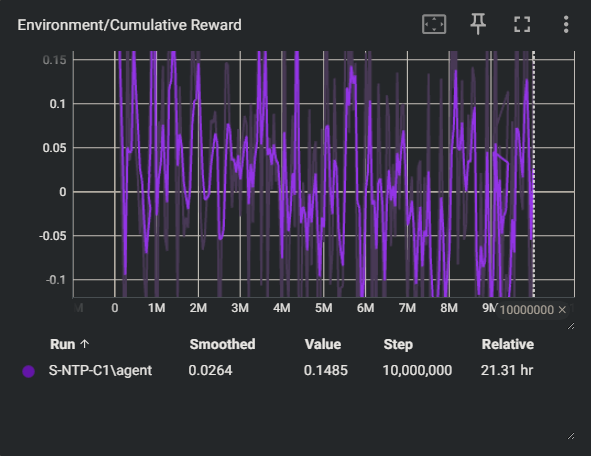
\includegraphics[width=\textwidth]{self-cumulative-reward.png}
        \caption{Αθροιστική ανταμοιβή (Πείραμα 3)}
        \label{fig:self-cumulative-reward}
    \end{minipage}
    \hfill
    \begin{minipage}[b]{0.48\textwidth}
        \centering
        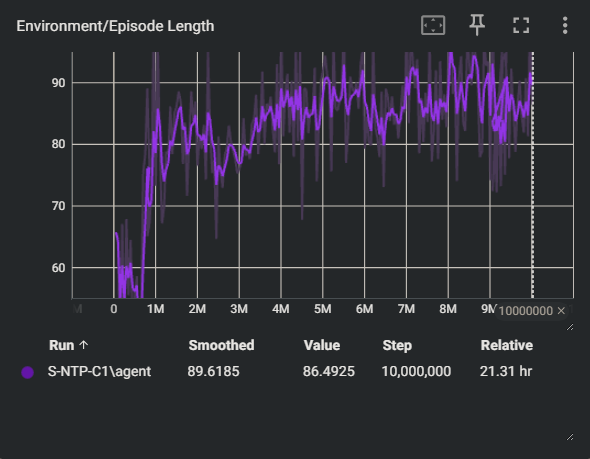
\includegraphics[width=\textwidth]{self-ep-duration.png}
        \caption{Διάρκεια επεισοδίου (Πείραμα 3)}
        \label{fig:self-ep-duration}
    \end{minipage}
\end{figure}

% 2. Στρατηγική Πυρομαχικών & Θερμοκρασίας (Πείραμα 3)
\begin{figure}[htbp]
    \centering
    \begin{minipage}[b]{0.48\textwidth}
        \centering
        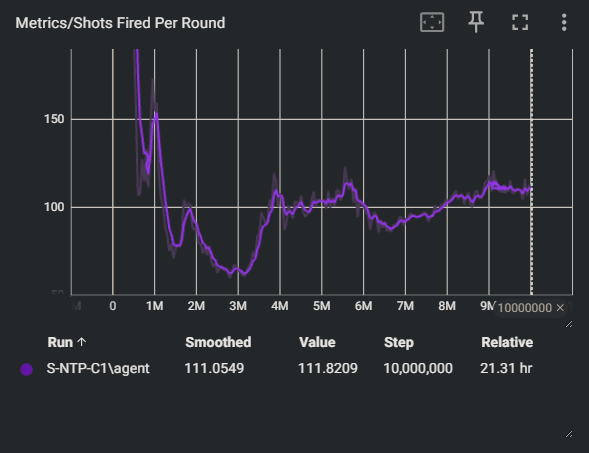
\includegraphics[width=\textwidth]{self-shots-per-round.png}
        \caption{Βολές ανά γύρο (Πείραμα 3)}
        \label{fig:self-shots-per-round}
    \end{minipage}
    \hfill
    \begin{minipage}[b]{0.48\textwidth}
        \centering
        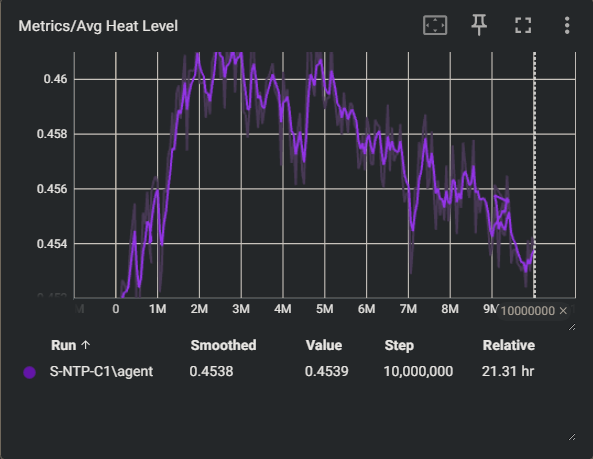
\includegraphics[width=\textwidth]{self-avg-heat.png}
        \caption{Μέση θερμοκρασία πράκτορα (Πείραμα 3)}
        \label{fig:self-avg-heat}
    \end{minipage}
\end{figure}

% 3. Σύγκριση Ακρίβειας (Πείραμα 3)
\begin{figure}[htbp]
    \centering
    \begin{minipage}[b]{0.48\textwidth}
        \centering
        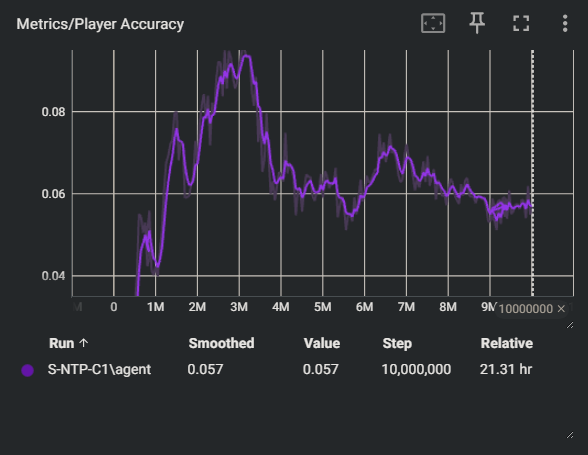
\includegraphics[width=\textwidth]{self-player-acc.png}
        \caption{Ακρίβεια βολών πράκτορα (Πείραμα 3)}
        \label{fig:self-player-acc}
    \end{minipage}
    \hfill
    \begin{minipage}[b]{0.48\textwidth}
        \centering
        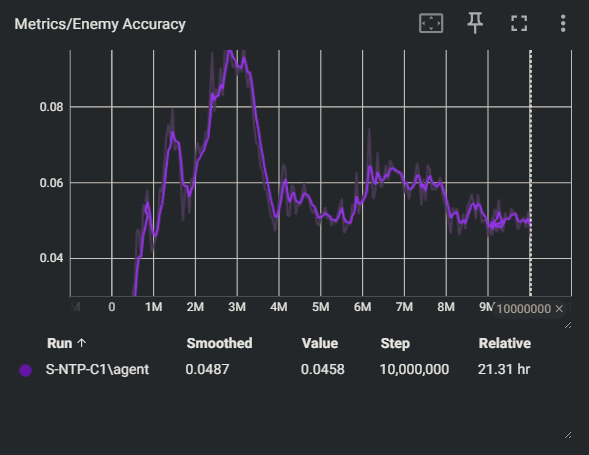
\includegraphics[width=\textwidth]{self-enemy-acc.png}
        \caption{Ακρίβεια βολών αντιπάλου (Πείραμα 3)}
        \label{fig:self-enemy-acc}
    \end{minipage}
\end{figure}

% 4. Αποτελεσματικότητα & Διάρκεια Νίκης (Πείραμα 3)
\begin{figure}[htbp]
    \centering
    \begin{minipage}[b]{0.48\textwidth}
        \centering
        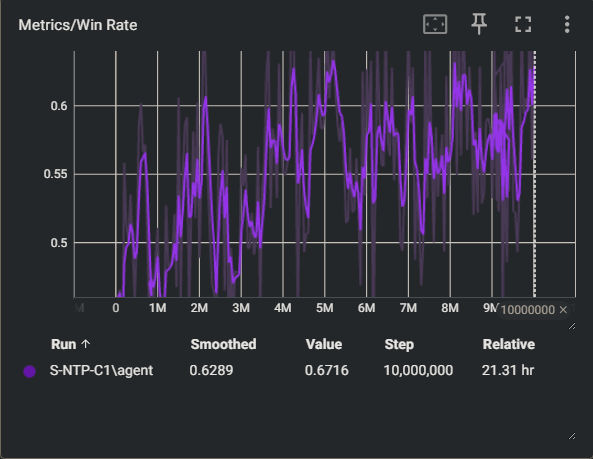
\includegraphics[width=\textwidth]{self-winrate.png}
        \caption{Αναλογία νίκης πράκτορα (Πείραμα 3)}
        \label{fig:self-winrate}
    \end{minipage}
    \hfill
    \begin{minipage}[b]{0.48\textwidth}
        \centering
        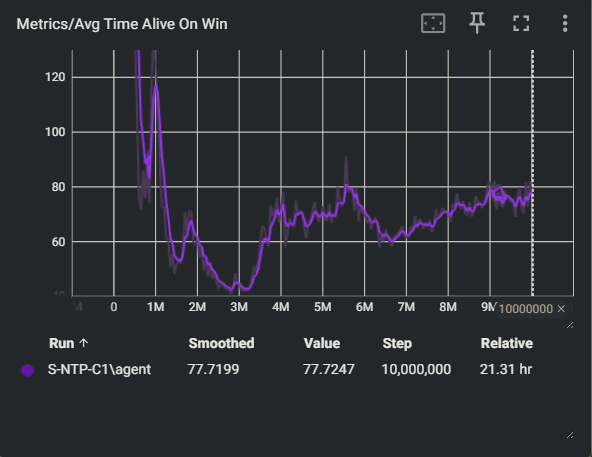
\includegraphics[width=\textwidth]{self-avg-dur-on-win.png}
        \caption{Διάρκεια επεισοδίου σε νίκη πράκτορα (Πείραμα 3)}
        \label{fig:self-avg-dur-on-win}
    \end{minipage}
\end{figure}

% 5. Εξέλιξη Εντροπίας (Πείραμα 3)
\begin{figure}[htbp]
    \centering
    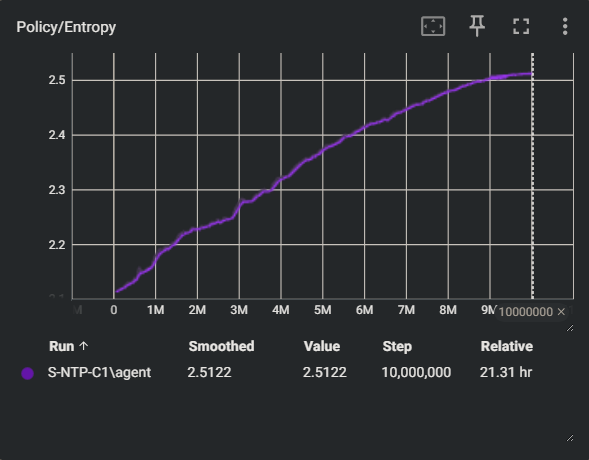
\includegraphics[width=0.48\textwidth]{self-entropy.png}
    \caption{Εντροπία πολιτικής (Πείραμα 3)}
    \label{fig:self-entropy}
\end{figure}

\subsection{PPO με Εξειδίκευμενη Αυτό-Εκπαίδευση (Fine-Tuning)}
Η αμυντική, και γενικότερα μη αποτελεσματική στρατηγική του πράκτορα, οδήγησε στην ιδέα του fine-tuning, μίας μεθόδου που χρησιμοποιείται ευρέως σε πολλά μοντέλα Μηχανικής Μάθησης, η οποία μπορεί μία γενική και υποβέλτιστη λύση, να την εξειδικεύσει και να παράξει μία.

% TODO: Finish sentence

\subsubsection{Κύριες Παράμετροι Πειράματος}
Βάσει της παραπάνω ιδέας, ως απόπειρα βελτίωσης του πράκτορα self-play, πραγματοποιήθηκε μια πρόσθετη φάση εξειδικευμένης εκπαίδευσης (fine-tuning), κατά την οποία ο ήδη εκπαιδευμένος πράκτορας self-play αρχικοποιήθηκε από την τελική του πολιτική και συνέχισε την εκπαίδευσή του για επιπλέον 1 εκατομμύριο βήματα, αυτή τη φορά εναντίον της απλής εκδοχής του πράκτορα βασισμένου σε κανόνες.

Η διαμόρφωση υπερπαραμέτρων διατήρησε το ίδιο μέγεθος δικτύου (512 μονάδες, 3 στρώματα) με την εκπαίδευση self-play, προϋπόθεση απαραίτητη για τη σωστή φόρτωση των ήδη εκπαιδευμένων βαρών του δικτύου, ενώ, πέρα από την αφαίρεση του self-play, δύο σημεία διαφοροποιήθηκαν σκόπιμα ώστε να ταιριάζουν στον χαρακτήρα προσαρμογής παρά πλήρους εκπαίδευσης. 

Αρχικά, ο ρυθμός μάθησης (learning rate) μειώθηκε από $3\cdot10^{-4}$ σε $1\cdot10^{-4}$, μια συνήθης πρακτική κατά το fine-tuning ήδη εκπαιδευμένων πολιτικών, η οποία αποσκοπεί στην αποφυγή απότομων, καταστροφικών ενημερώσεων που θα μπορούσαν να διαταράξουν την ήδη αναπτυγμένη ικανότητα στόχευσης του πράκτορα, επιτρέποντας αντ' αυτού πιο σταδιακή, προσαρμογή της υπάρχουσας συμπεριφοράς στα νέα δεδομένα του στατικού αντιπάλου. 

Στη συνέχεια το πρόγραμμα μεταβολής του συντελεστή εντροπίας (beta schedule) τροποποήθηκε από σταθερό σε γραμμικό, αφού η σταθερότητα χρησιμοποίηθηκε στο self-play για την αποφυγή πρόωρης σύγκλισης του πράκτορα σε μια στενή, εξειδικευμένη συμπεριφορά την οποία θα αναγκαζόταν να ξαναμάθει από την αρχή κάθε φορά που άλλαζε η συμπεριφορά του αντιπάλου.

% TODO: Add parameter list and finish paragraph with more sensible config

\begin{table}[H]
	\centering
	\caption{Διαμόρφωση Υπερπαραμέτρων Fine-Tune (Βασική Εκδοχή)}
	\label{tab:ft-base-params}
	\begin{tabular}{ll}
		\hline
		\textbf{Υπερπαράμετρος} & \textbf{Τιμή} \\
		\hline
		Learning rate & $1 \cdot 10^{−4}$ (linear schedule) \\
		Epsilon (clip) & 0.2 (linear schedule) \\
		Beta (entropy coefficient) & 0.01 (linear schedule) \\
		Number of epochs & 3 \\
		Hidden units & 512 \\
		Number of hidden layers & 3 \\
		Gamma (discount factor) & 0.99 \\
		Time horizon & 128 \\
		\hline
	\end{tabular}
\end{table}

\subsubsection{Αποτελέσματα Πειράματος}
Λόγω της συμμετρικής φύσης του self-play, όπου οι πράκτορες εξελίσσονται παράλληλα, οι περισσότερες μετρικές ταλαντώνονται γύρω από σχετικά σταθερές τιμές χωρίς σαφή τάση σύγκλισης (Αναλογία Νίκης: 45\%–65\%, Αθροιστική Ανταμοιβή: -0.1 εώς 0.15). Στην περίπτωση του fine-tuning, αντίθετα, παρατηρείται ξεκάθαρη σύγκλιση σε αρκετά διαγράμματα, με χαρακτηριστικότερα την αθροιστική ανταμοιβή (από 0.75 σε 1.64) και την αναλογία νίκης του πράκτορα (από 68\% σε 96\%). Παράλληλα, η ισορροπία που προϋπήρχε στην ακρίβεια βολών μεταξύ πράκτορα και αντιπάλου έχει καταρρεύσει υπέρ του πρώτου (από ~5\% σε 33\% έναντι 11\%).

Ποιοτικά, ο πράκτορας διατηρεί σε μεγάλο βαθμό την ήδη εκμαθημένη διαδικασία στόχευσης, ενώ η συγκριτικά ασθενέστερη αμυντική του ικανότητα έχει βελτιωθεί σημαντικά. Παρατηρείται επίσης ότι η συμπεριφορά του πλέον ενσωματώνει ελιγμούς αποφυγής βολών και συνεχή κίνηση, υποδεικνύοντας ότι ο πράκτορας έχει αναπτύξει ικανότητα επιβίωσης απέναντι σε πιο επιθετικούς αντιπάλους. Η αξιολόγηση του πράκτορα έναντι της σύνθετης εκδοχής του αντιπάλου παράγει αντίστοιχα αποτελέσματα επικράτησης και υψηλό ποσοστό νίκης, γεγονός που καταδεικνύει ικανοποιητική ικανότητα γενίκευσης απέναντι σε στρατηγικές με τις οποίες δεν έχει αλληλεπιδράσει άμεσα κατά την εκπαίδευση. Η συνολική στρατηγική του, ωστόσο, παραμένει σε μεγάλο βαθμό αμυντικού χαρακτήρα, καθώς προτιμά να αναμένει την είσοδο του αντιπάλου εντός της μέγιστης εμβέλειας πριν πυροβολήσει, διατηρώντας σχετικά ασφαλή απόσταση, επιλογή που του παρέχει περισσότερο χρόνο για αποφυγή εισερχόμενων βολών.

\subsubsection{Γραφήματα Αποτελεσμάτων}
% Ζεύγος 1: Αθροιστική Ανταμοιβή & Μέση Διάρκεια Επεισοδίου (Πείραμα 4)
\begin{figure}[H]
	\centering
	\begin{minipage}[b]{0.48\textwidth}
		\centering
		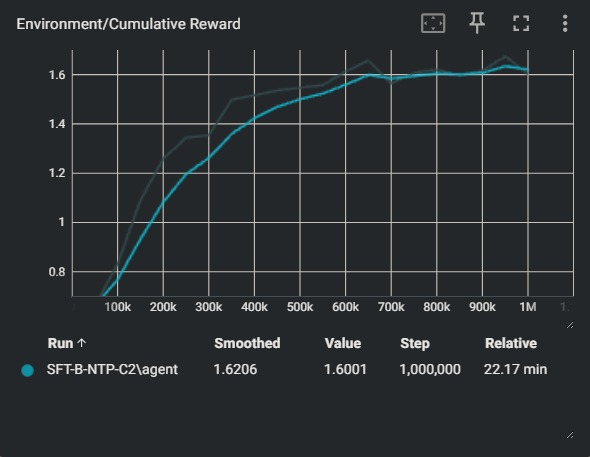
\includegraphics[width=\textwidth]{self-ft-cumulative-reward}
		\caption{Αθροιστική ανταμοιβή πράκτορα (Πείραμα 4)}
		\label{fig:self-ft-cumulative-reward}
	\end{minipage}
	\hfill
	\begin{minipage}[b]{0.48\textwidth}
		\centering
		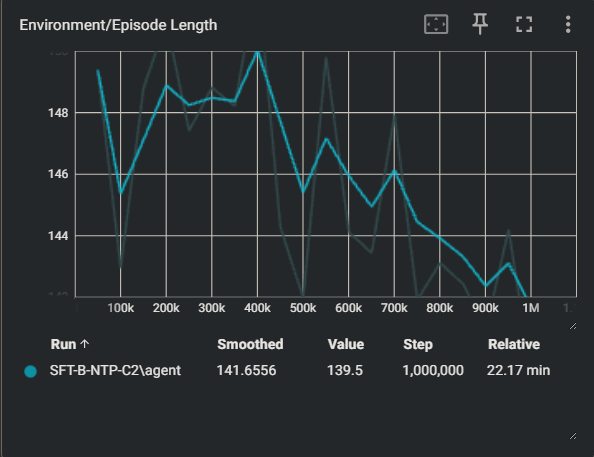
\includegraphics[width=\textwidth]{self-ft-ep-duration}
		\caption{Μέση διάρκεια επεισοδίου (Πείραμα 4)}
		\label{fig:self-ft-ep-duration}
	\end{minipage}
\end{figure}

% Ζεύγος 2: Μέση Θερμοκρασία & Βολές (Πείραμα 4)
\begin{figure}[H]
	\centering
	\begin{minipage}[b]{0.48\textwidth}
		\centering
		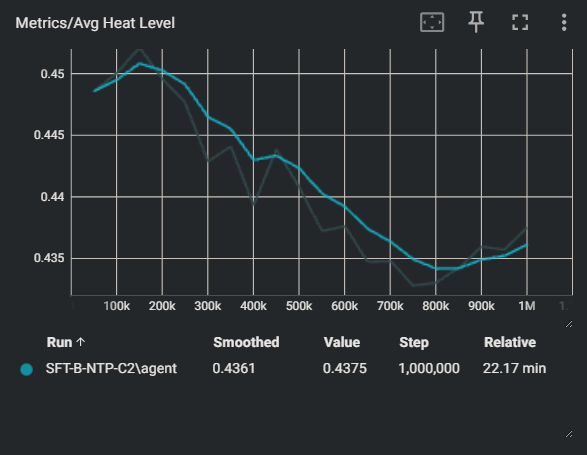
\includegraphics[width=\textwidth]{self-ft-avg-heat}
		\caption{Μέση θερμοκρασία πράκτορα (Πείραμα 4)}
		\label{fig:self-ft-avg-heat}
	\end{minipage}
	\hfill
	\begin{minipage}[b]{0.48\textwidth}
		\centering
		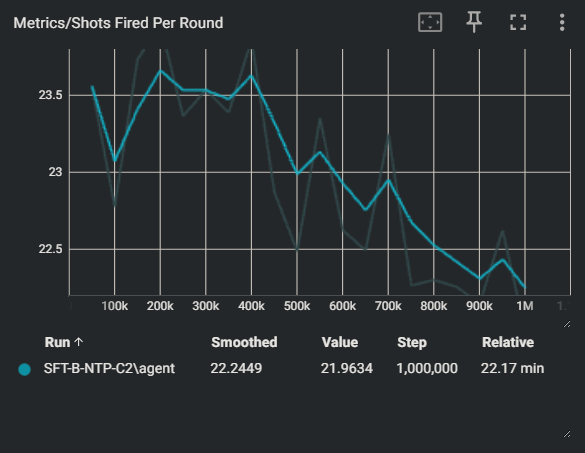
\includegraphics[width=\textwidth]{self-ft-shots-fired}
		\caption{Συνολικός αριθμός βολών (Πείραμα 4)}
		\label{fig:self-ft-shots-fired}
	\end{minipage}
\end{figure}

% Ζεύγος 3: Ακρίβεια Αντιπάλου & Ακρίβεια Πράκτορα (Πείραμα 4)
\begin{figure}[H]
	\centering
	\begin{minipage}[b]{0.48\textwidth}
		\centering
		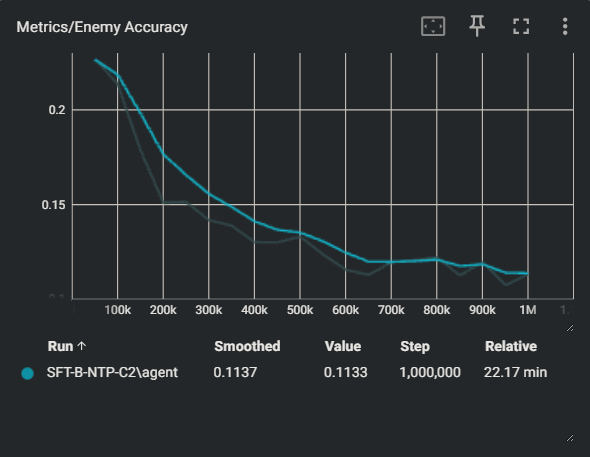
\includegraphics[width=\textwidth]{self-ft-enemy-acc}
		\caption{Ακρίβεια βολών αντιπάλου (Πείραμα 4)}
		\label{fig:self-ft-enemy-acc}
	\end{minipage}
	\hfill
	\begin{minipage}[b]{0.48\textwidth}
		\centering
		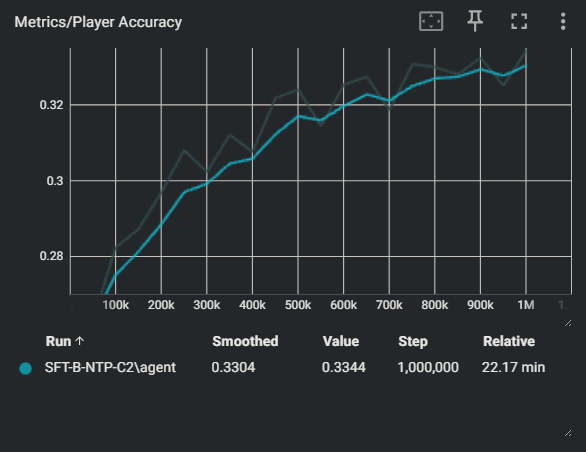
\includegraphics[width=\textwidth]{self-ft-player-acc}
		\caption{Ακρίβεια βολών πράκτορα (Πείραμα 4)}
		\label{fig:self-ft-player-acc}
	\end{minipage}
\end{figure}

% Ζεύγος 4: Αναλογία Νίκης & Εντροπία Πολιτικής (Πείραμα 4)
\begin{figure}[H]
	\centering
	\begin{minipage}[b]{0.48\textwidth}
		\centering
		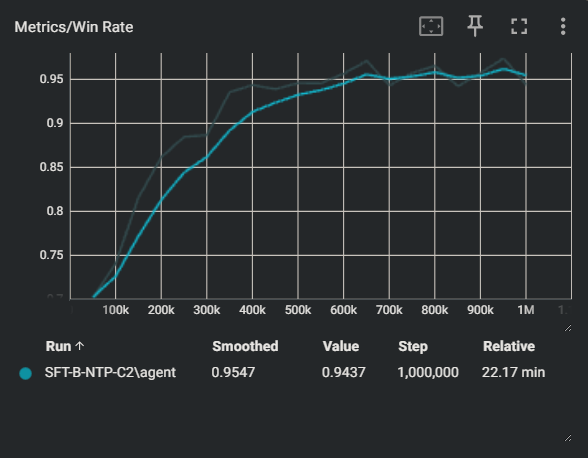
\includegraphics[width=\textwidth]{self-ft-winrate}
		\caption{Αναλογία νίκης πράκτορα (Πείραμα 4)}
		\label{fig:self-ft-winrate}
	\end{minipage}
	\hfill
	\begin{minipage}[b]{0.48\textwidth}
		\centering
		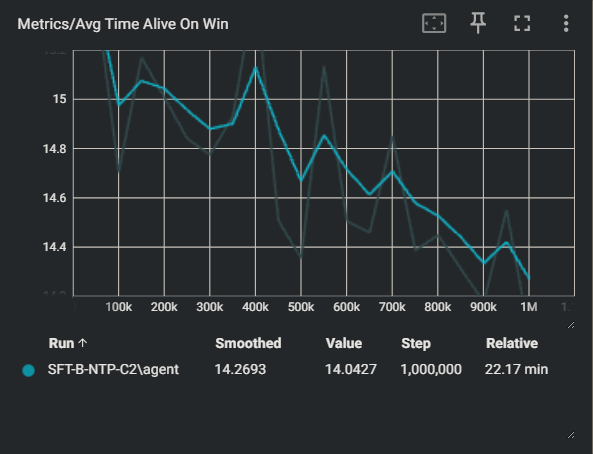
\includegraphics[width=\textwidth]{self-ft-dur-on-win}
		\caption{Διάρκεια επεισοδίου σε νίκη πράκτορα (Πείραμα 4)}
		\label{fig:self-ft-dur-on-win}
	\end{minipage}
\end{figure}

% 9. Διάρκεια Επεισοδίου σε Νίκη Πράκτορα (Πείραμα 4)
\begin{figure}[H]
	\centering
	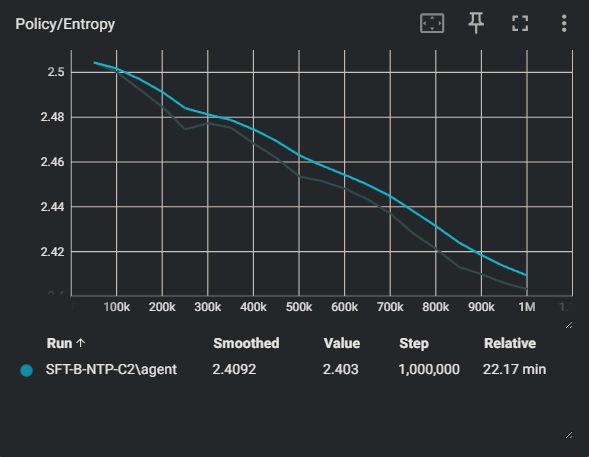
\includegraphics[width=0.48\textwidth]{self-ft-entropy}
	\caption{Εντροπία πολιτικής (Πείραμα 4)}
	\label{fig:self-ft-entropy}
\end{figure}

\subsection{Σύγκριση Αποτελεσμάτων}
Παρακάτω συγκρίνονται οι χρόνοι εκπαίδευσης των διαφορετικών πειραμάτων που αναλύθηκαν, καθώς και σχετικές παράμετροι. Στην εκπαίδευση του self-play το ML-Agents Toolkit απέτυχε να παραλληλοποιήσει την διαδικασία εκπαίδευσης, προσφέροντας μηδενικό speedup για 8 περιβάλλοντα.

\begin{table}[H]
	\centering
	\caption{Συγκριτικός πίνακας παραμέτρων και απόδοσης εκπαίδευσης πειραμάτων}
	\label{tab:experiments_summary}
	\resizebox{\textwidth}{!}{%
		\begin{tabular}{|l|c|c|c|c|}
			\hline
			\textbf{Πείραμα} & \textbf{Βήματα / δευτερόλεπτο} & \textbf{Αριθμός περιβαλλόντων} & \textbf{Συνολικός χρόνος εκπαίδευσης} & \textbf{Αριθμός βημάτων} \\
			\hline
			PPO vs Baseline & 714 steps / sec & 8 & ~7000 seconds & 5 million \\
			\hline
			PPO vs Baseline & 714 steps / sec & 8 & ~14000 seconds & 10 million \\
			\hline
			PPO vs Advanced & 714 steps / sec & 8 & ~14000 seconds & 10 million \\
			\hline
			PPO Self Play & 277 steps / sec & 1 & ~55400 seconds & 10 million \\
			\hline
			PPO Fine Tune & 714 steps / sec & 8 & ~1400 seconds & 1 million \\
			\hline
		\end{tabular}%
	}
\end{table}

Το Self-Play, σε γενικές γραμμές, έχει μεγαλύτερη διάρκεια εκπαίδευσης λόγω overhead, η δυναμικότητά του όμως προέρχεται από την χρήση του στην παραγωγή διαφορετικών fine-tuned πρακτόρων σε πολύ σύντομο χρονικό διάστημα.

\section{Συμπεράσματα}
Τα αποτελέσματα της πειραματικής αξιολόγησης δείχνουν ότι οι σύγχρονες μέθοδοι
Ενισχυτικής Μάθησης, και συγκεκριμένα ο αλγόριθμος PPO, είναι σε θέση όχι μόνο
να νικήσουν με συνέπεια πράκτορες βασισμένους σε κανόνες,
αλλά και να αναπτύξουν, μέσα από την ίδια τη διαδικασία εκπαίδευσης, συμπεριφορές
που θα θεωρούνταν χαρακτηριστικές ενός χειροκίνητα σχεδιασμένου πράκτορα (π.χ.
διαχείριση πόρων, χρήση κάλυψης, αποφυγή βλημάτων, στόχευση αντιπάλου). Το
γεγονός αυτό είναι ιδιαίτερα σημαντικό, καθώς οι συμπεριφορές αυτές προέκυψαν
χωρίς καμία ρητή, χειροκίνητη κωδικοποίηση λογικής (όπως θα απαιτούσε μια FSM)
και χωρίς την ανάγκη μιας χρονοβόρας διαδικασίας reward shaping,
αντιθέτως, χρησιμοποιήθηκε ένα ελάχιστο, αραιό σύνολο ανταμοιβών.

Το εύρημα αυτό υποδεικνύει ότι η Ενισχυτική Μάθηση αποτελεί μια απολύτως
βιώσιμη επιλογή για την ανάπτυξη πρακτόρων παιχνιδιών με σχετικά μικρό κόπο και
χωρίς εκτενή εμπειρογνωμοσύνη στον σχεδιασμό κανόνων συμπεριφοράς εκ μέρους
του προγραμματιστή. Παρέχει, επιπλέον, ένα σημαντικό πλεονέκτημα προσαρμοστικότητας
έναντι των παραδοσιακών πρακτόρων, αφού η ίδια βασική μεθοδολογία μπορεί να
εφαρμοστεί σε διαφορετικά σενάρια ή περιβάλλοντα απλώς μέσω επανεκπαίδευσης,
χωρίς την ανάγκη επανασχεδιασμού της λογικής του πράκτορα από την αρχή.
Παράλληλα, τεχνικές όπως το self-play και το μεταγενέστερο fine-tuning
φάνηκαν ικανές να βελτιώσουν περαιτέρω τόσο τη γενικευσιμότητα όσο και την
τελική απόδοση του πράκτορα, με σχετικά μικρό πρόσθετο υπολογιστικό κόστος.

Συνολικά, τα αποτελέσματα της παρούσας εργασίας ενισχύουν την άποψη ότι οι πράκτορες RL μπορούν να
αποτελέσουν μια ρεαλιστική, πρακτική εναλλακτική στους καθιερωμένους rule-based
πράκτορες για την ανάπτυξη τεχνητής νοημοσύνης σε παιχνίδια με δυναμικά περιβάλλοντα, ακόμα και υπό
συνθήκες περιορισμένης ανθρώπινης παρέμβασης και με τη χρήση σχετικά απλών μεθόδων εκπαίδευσης.

\pagebreak

\bibliographystyle{apalike}
\bibliography{mybib}

\end{document}
